% ============================================================
%  Projeto Integrativo 3 — Projeto 3, entrega Q1
%  Modelos autorregressivos e de classificação para detecção de queda
%  Escola Politécnica da USP
%
%  Tabelas (tabelas/) e figuras (figuras/) são geradas por
%  modelo/experimentos/08_relatorio_latex.py a partir de modelo/resultados/.
% ============================================================
\documentclass[12pt,a4paper]{article}

% --- Encoding & Language ---
\usepackage[utf8]{inputenc}
\usepackage[T1]{fontenc}
\usepackage[brazilian]{babel}
\usepackage{lmodern}

% --- Colors ---
\usepackage{xcolor}
\definecolor{uspblue}{RGB}{0,84,166}
\definecolor{lightblue}{RGB}{220,235,248}

% --- TOC (antes do parskip, que também mexe no sumário) ---
\usepackage{tocloft}
\renewcommand{\cftsecfont}{\bfseries\color{uspblue}}
\renewcommand{\cftsecpagefont}{\bfseries\color{uspblue}}
\setlength{\cftbeforesecskip}{4pt}

% --- Layout ---
\usepackage[
  a4paper,
  top=3cm, bottom=2cm,
  left=3cm, right=2cm,
  headheight=25pt
]{geometry}
\usepackage{parskip}
\setlength{\parindent}{0pt}
\setlength{\parskip}{6pt}
\setlength{\emergencystretch}{1.5em}

% --- Math ---
\usepackage{amsmath,amssymb}

% --- Tables ---
\usepackage{booktabs,makecell,array}
\usepackage{siunitx}
\sisetup{output-decimal-marker={,}, exponent-product=\times, group-digits=false,
         retain-explicit-plus=false}

% --- Images ---
\usepackage{graphicx}
\usepackage{float}

% --- Headers & Footers ---
\usepackage{fancyhdr}
\pagestyle{fancy}
\fancyhf{}
\fancyhead[L]{\small\textcolor{uspblue}{EPUSP - Projeto Integrativo 3}}
\fancyhead[R]{\small\textcolor{uspblue}{\thepage}}
\fancyfoot[C]{}
\renewcommand{\headrulewidth}{0.4pt}
\renewcommand{\headrule}{\hbox to\headwidth{\color{uspblue}\leaders\hrule height \headrulewidth\hfill}}

% --- Section Styling ---
\usepackage{titlesec}
\titleformat{\section}
  {\large\bfseries\color{uspblue}}
  {\thesection.}{0.6em}{}
  [\vspace{-5pt}\textcolor{uspblue}{\rule{\linewidth}{0.4pt}}\vspace{1pt}]
\titleformat{\subsection}
  {\normalsize\bfseries\color{uspblue!80!black}}
  {\thesubsection}{0.6em}{}
\titleformat{\subsubsection}
  {\normalsize\bfseries}
  {\thesubsubsection}{0.6em}{}

% --- Caption ---
\usepackage{caption}
\captionsetup{
  font=small,
  labelfont={bf,color=uspblue},
  labelsep=period,
}
\captionsetup[table]{position=top}

% --- Lists ---
\usepackage{enumitem}
\setlist[itemize]{noitemsep, topsep=4pt}
\setlist[enumerate]{noitemsep, topsep=4pt}

% --- Hyperref (por último) ---
\usepackage[
  colorlinks=true,
  linkcolor=uspblue,
  urlcolor=uspblue,
  citecolor=uspblue,
  bookmarks=true,
  pdftitle={Projeto Integrativo 3 - Projeto 3 - Q1},
  pdfauthor={Dimitri Garcia, Henrique Guimarães Margarido, Henrique Santiago},
]{hyperref}

% --- Macros ---
\newcommand{\code}[1]{\texttt{#1}}
\newcommand{\amag}{|a|}
\newcommand{\wmag}{|\omega|}
% Docentes da disciplina: preencha para a linha aparecer na contracapa.
\newcommand{\docentes}{}

\begin{document}
	\pagenumbering{Alph}
	% ============================================================
	%  CAPA
	% ============================================================
	\begin{titlepage}
		\centering

		
\includegraphics[scale=0.25]{imagens/Logo-Escola-Politecnica.jpg}

		\vspace{0.3cm}

		{\Large\bfseries UNIVERSIDADE DE S\~AO PAULO}\\[0.3cm]
		{\large ESCOLA POLIT\'ECNICA}\\[0.2cm]

		\vspace{1.4cm}

		\begin{tabular}{p{10cm}l}
			DIMITRI GARCIA & NUSP 1682224 \\
			HENRIQUE GUIMAR\~AES MARGARIDO & NUSP 5797753 \\
			HENRIQUE SANTIAGO & NUSP 16872729 \\
		\end{tabular}

		\vspace{1.3cm}
		\textcolor{uspblue}{\rule{\linewidth}{1.5pt}}
		\vspace{0.3cm}

		{\LARGE\bfseries\color{uspblue} PROJETO 3 --- ENTREGA Q1}\\[0.5cm]
		{\large\itshape Modelos autorregressivos e de classificação \\[0.2cm]
			para a detecção de quedas no vestível}

		\vspace{0.4cm}
		\textcolor{uspblue}{\rule{\linewidth}{1.5pt}}

		\vfill
		\begin{tabular}{p{3.5cm}l}
			\textbf{Disciplina:} & 0323221 - Projeto Integrativo 3 \\[0.2cm]
			\textbf{Data:} & 10 de novembro de 2026 \\[0.2cm]
			\textbf{Local:} & S\~ao Paulo \\
		\end{tabular}

		\vfill
		\phantom{fim}
	\end{titlepage}

	% ============================================================
	%  CONTRACAPA
	% ============================================================
	\begin{titlepage}
		\centering

		{\large DIMITRI GARCIA\\HENRIQUE GUIMAR\~AES MARGARIDO\\HENRIQUE SANTIAGO\\}

		\vspace{4cm}
		{\LARGE{PROJETO 3 --- ENTREGA Q1}} \\
		\vspace{2cm}
		\begin{flushright}
			\begin{minipage}{0.55\textwidth}
				Entrega referente à disciplina 0323221 - Projeto Integrativo 3 (2026),
				Projeto 3, quesito Q1: desenvolvimento do modelo autorregressivo e dos
				modelos de classificação. \\[0.5cm]
				Desenvolvimento e comparação, no computador, de modelos que decidem se
				houve queda a partir do acelerômetro e do giroscópio do vestível do
				sistema de monitoramento de idosos: pipeline com filtro, gatilho e
				janela; modelos autorregressivos AR e ARX; correlação cruzada com
				templates; DTW; atributos no tempo e em frequência; distâncias;
				classificadores e rede convolucional; avaliação por pessoa na base
				pública SisFall e teste em ensaios próprios.
				\ifx\docentes\empty\else\\[0.5cm]\textbf{Docentes:} \docentes.\fi
			\end{minipage}
		\end{flushright}

		\vfill
		{\small Escola Polit\'ecnica da USP --- S\~ao Paulo, 10 de novembro de 2026}
	\end{titlepage}
	\pagenumbering{arabic}

	% ============================================================
	%  RESUMO
	% ============================================================
	\section*{Resumo}
	O vestível do nosso sistema de monitoramento de idosos detecta quedas hoje por um
	limiar provisório de 2,5\,g na magnitude da aceleração. Correr, pular e sentar com
	força também passam desse limiar. Este relatório desenvolve e compara, no
	computador, os modelos que vão substituí-lo. O limiar vira um \emph{gatilho} que
	só acorda o classificador; uma janela de 1,8\,s em torno do pico de $\amag$ é
	então classificada como queda ou não queda. Testamos 22 métodos: os das aulas
	(modelos autorregressivos AR e ARX, correlação cruzada normalizada e não
	normalizada, DTW, atributos no tempo e em frequência, distâncias) e os usuais na
	literatura (regras, regressão logística, árvore, SVM, Random Forest e CNN 1D).
	Na base pública SisFall, com validação cruzada por pessoa e o sensor na faixa do
	vestível ($\pm$8\,g), o limiar atual dá 69,9 alarmes falsos por hora de atividade;
	com cerca de 94\,\% das quedas detectadas, o Random Forest dá 0,4 e a regressão
	logística, com um modelo de 412 bytes, 1,4. O que separa a queda de uma corrida
	não é o tamanho do pico, e sim a queda livre antes e a postura e a quietude
	depois do impacto. O AR descreve bem a atividade normal, mas, como detector de
	anomalia, também dispara em qualquer movimento brusco (AUC 0,79). Nos nossos 18
	ensaios, os modelos de atributos não deram nenhum alarme ao andar ou correr, mas
	perderam as quedas de joelhos.

	{\raggedright
	\textbf{Palavras-chave:} detecção de queda; modelo autorregressivo; classificação;
	correlação cruzada; DTW; Random Forest; acelerômetro; ESP32.\par}

	\newpage
	\tableofcontents
	\thispagestyle{fancy}
	\newpage

%======================================================================
\section{Introdução}\label{sec:intro}
%======================================================================
O sistema monitora idosos em Instituições de Longa Permanência (ILPIs) de forma não
invasiva. Em cada quarto, um hub com ESP32-S3 lê portas, presença e temperatura, roda
as regras de alerta e publica tudo por MQTT. O idoso usa um vestível, também com
ESP32-S3 e um acelerômetro e giroscópio MPU-6050, que detecta quedas e avisa o hub.

O detector de quedas atual é \textbf{provisório}: ele dispara quando $\amag^2$ passa
de 6,25\,g$^2$ ($\amag > 2{,}5$\,g), com histerese. Ele pega as quedas, mas também
correr, pular, subir escada rápido ou sentar com força: todos esses movimentos passam
de 2,5\,g. O Q1 do Projeto 3 pede o desenvolvimento do modelo autorregressivo e dos
modelos de classificação. Nesta entrega, desenvolvemos e comparamos esses modelos
\textbf{no computador}, antes de levá-los ao ESP32.

\paragraph{Binário ou caracterizador?} A saída é \textbf{binária}: queda ou não queda.
O alarme só precisa saber se houve queda. Um classificador dos 15 tipos de queda da
SisFall dividiria os dados em classes de cerca de 120 exemplos e erraria mais
justamente no que importa. Os tipos de queda e de atividade entram na análise dos
erros (Seção~\ref{sec:erros}). Perder uma queda é pior que um alarme falso, e o botão
``estou bem'' do vestível já cancela alarmes falsos; por isso o ponto de operação
privilegia a sensibilidade.

\paragraph{Organização.} A Seção~\ref{sec:dados} descreve os dados; a
Seção~\ref{sec:pipeline}, o pipeline comum a todos os métodos; a
Seção~\ref{sec:modelos}, os modelos; a Seção~\ref{sec:avaliacao}, a avaliação e os
testes; a Seção~\ref{sec:resultados}, os resultados; e as
Seções~\ref{sec:discussao} e \ref{sec:conclusoes}, a discussão e as conclusões. O
Apêndice~\ref{ap:reproducao} explica como reproduzir tudo.

%======================================================================
\section{Dados}\label{sec:dados}
%======================================================================
\begin{table}[H]
\centering
\caption{Bases usadas. Nas duas, o sensor fica na cintura.}
\label{tab:dados}
\small
\begin{tabular}{@{}l>{\raggedright\arraybackslash}p{4.2cm}>{\raggedright\arraybackslash}p{4.4cm}>{\raggedright\arraybackslash}p{3.2cm}@{}}
\toprule
Base & Pessoas & Ensaios & Sensor e taxa \\
\midrule
SisFall \cite{sisfall} & 38: 23 jovens e 15 idosos (os idosos só fazem atividades, exceto um); 24 fizeram quedas
  & 4505: 2707 atividades de 19 tipos (14,5\,h) e 1798 quedas de 15 tipos (7,5\,h)
  & ADXL345 $\pm$16\,g e ITG3200 $\pm$2000\,°/s, 200\,Hz \\
Nossa & 1 & 18: andar (4), correr (4), queda de costas (3), de frente (4) e de joelhos (3)
  & MPU-6050 $\pm$2\,g e $\pm$250\,°/s, $\approx$193\,Hz \\
\bottomrule
\end{tabular}
\end{table}

\paragraph{SisFall.} A base foi conferida antes do uso: os 4505 arquivos têm 9
colunas e nenhum está vazio. Os valores brutos são convertidos para g e °/s
($2\cdot16/2^{13}$\,g e $2\cdot2000/2^{16}$\,°/s por unidade). A pessoa é lida pela
pasta, e não pelo nome do arquivo, porque cinco ensaios da SA15 foram gravados com o
nome \code{D17\_SE15}.

\paragraph{Nossos ensaios.} Foram gravados com o vestível preso à cintura, por uma
pessoa. Os arquivos não têm cabeçalho e já estão em g e °/s; o tempo tem resolução de
10\,ms, então foi reconstruído como uniforme e os sinais foram reamostrados para
200\,Hz. Os ensaios são curtos (1,9 a 5,5\,s), com só 0,8 a 1,6\,s depois do impacto.
O sensor estava em $\pm$2\,g e satura em todos os arquivos: o $\amag$ máximo é
$2\sqrt3\approx3{,}46$\,g.

\paragraph{Dois cenários de faixa.} Para comparar com o vestível, a SisFall é saturada
eixo a eixo em duas faixas:
\begin{itemize}[leftmargin=1.5em]
\item \textbf{A:} $\pm$8\,g e $\pm$500\,°/s, a configuração atual do firmware. É a
  comparação principal.
\item \textbf{B:} $\pm$2\,g e $\pm$250\,°/s, a dos nossos ensaios. Os modelos testados
  neles são treinados na SisFall saturada em B.
\end{itemize}
A Figura~\ref{fig:sinais} mostra sinais típicos, e a Figura~\ref{fig:saturacao}, o
efeito da saturação: em $\pm$2\,g, os picos de uma queda e de uma corrida ficam quase
iguais.

\begin{figure}[H]
  \centering
  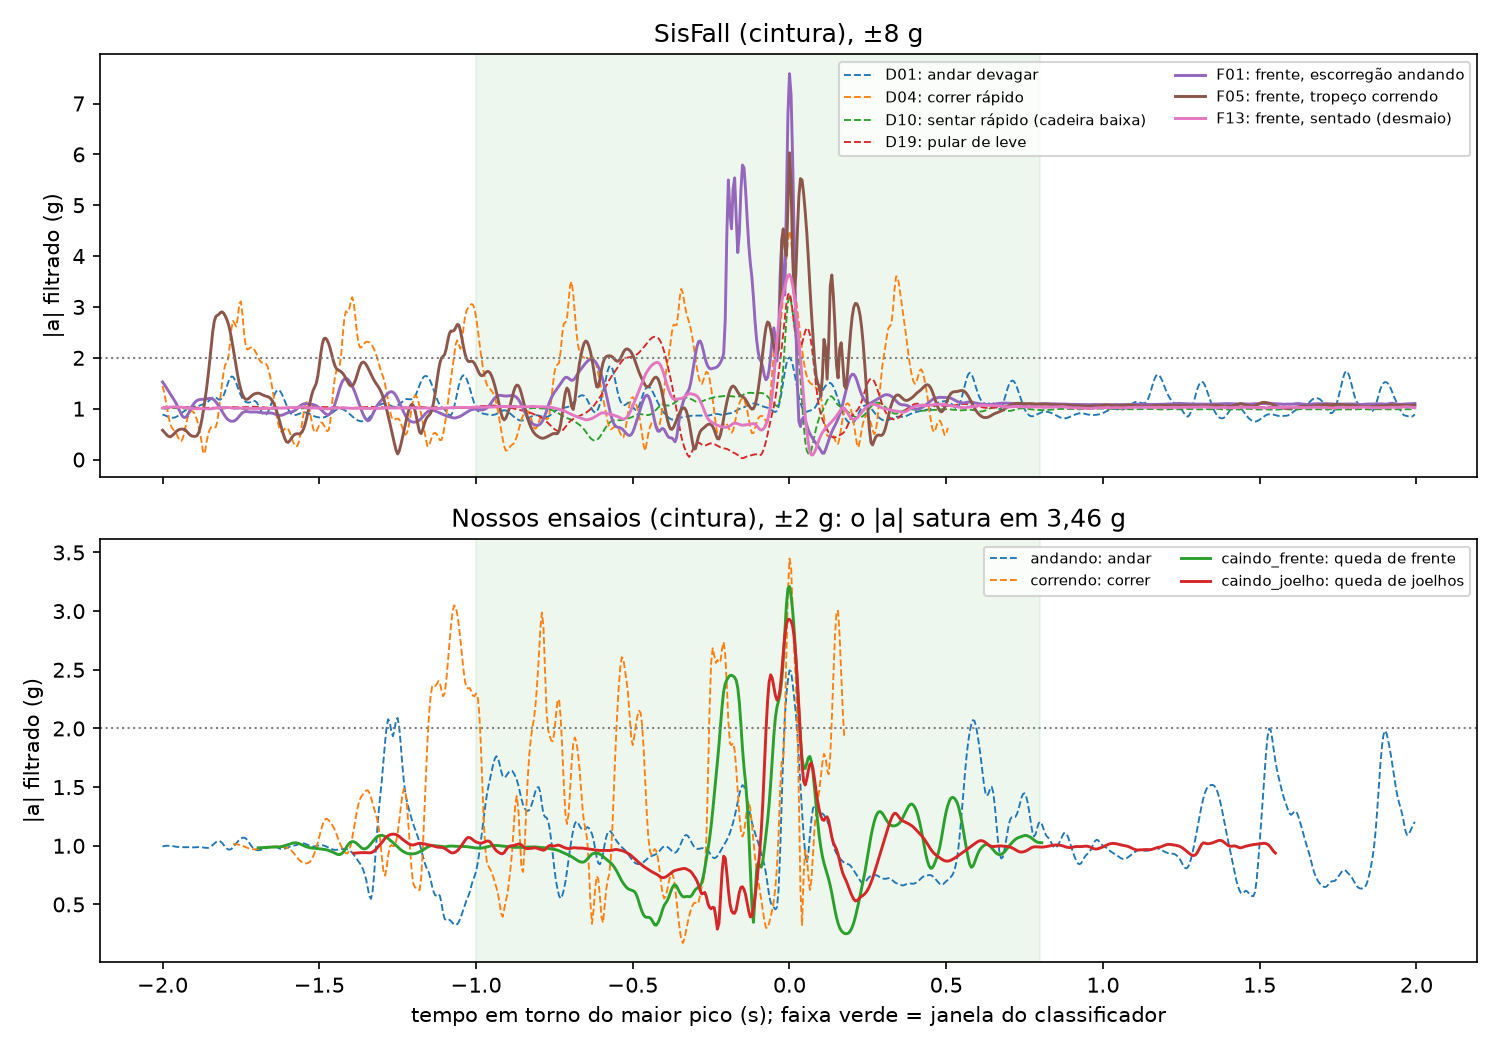
\includegraphics[width=0.92\linewidth]{figuras/fig_sinais.png}
  \caption{$\amag$ filtrado de atividades (tracejado) e quedas (contínuo), centrado no
  maior pico. Acima, a SisFall no cenário A; abaixo, nossos ensaios, saturados em
  3,46\,g. A faixa verde é a janela que vai para o classificador
  (Seção~\ref{sec:pipeline}); a linha pontilhada, o gatilho de 2,0\,g.}
  \label{fig:sinais}
\end{figure}

\begin{figure}[H]
  \centering
  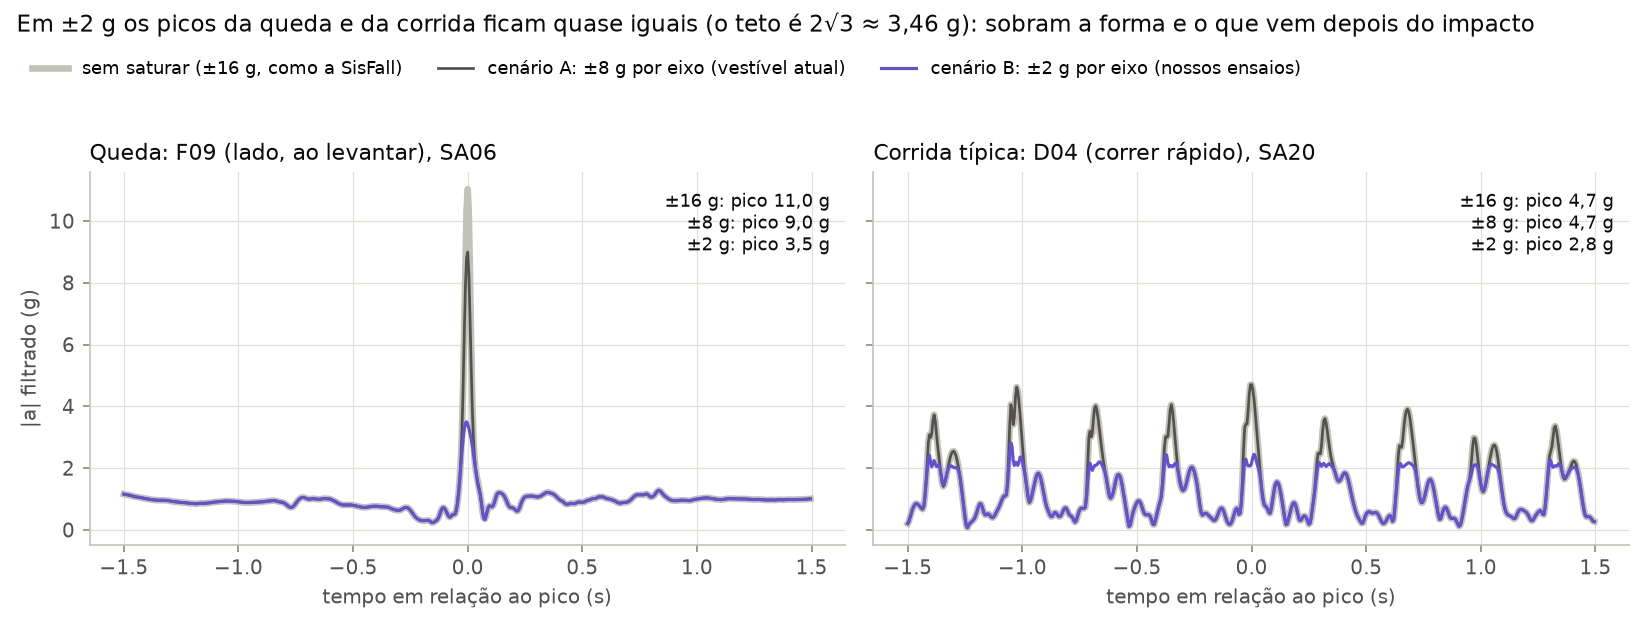
\includegraphics[width=\linewidth]{figuras/fig_saturacao.png}
  \caption{A mesma queda e a mesma corrida da SisFall sem saturar ($\pm$16\,g) e
  saturadas nos cenários A e B. Em $\pm$2\,g, o pico deixa de distinguir a queda.}
  \label{fig:saturacao}
\end{figure}

%======================================================================
\section{Pipeline de detecção}\label{sec:pipeline}
%======================================================================
Todos os métodos recebem as mesmas janelas, produzidas pelo pipeline abaixo, que é o
que vai rodar no vestível:
\begin{enumerate}[leftmargin=1.8em]
\item \textbf{Magnitude e filtro.} $\amag=\sqrt{a_x^2+a_y^2+a_z^2}$ e
  $\wmag=\sqrt{\omega_x^2+\omega_y^2+\omega_z^2}$, depois de um passa-baixa
  Butterworth de 2.ª ordem em 20\,Hz, causal. É um único biquad, como o
  \code{dsps\_biquad\_f32} do ESP-DSP:
  \begin{equation}\label{eq:biquad}
    y[n]=b_0x[n]+b_1x[n-1]+b_2x[n-2]-a_1y[n-1]-a_2y[n-2].
  \end{equation}
\item \textbf{Gatilho.} Os picos de $\amag$ acima de $L_\text{on}$, separados por pelo
  menos 0,5\,s. O gatilho \emph{não decide} a queda: só acorda o classificador.
\item \textbf{Janela} de 1,0\,s antes a 0,8\,s depois do pico (360 amostras a
  200\,Hz). Antes do pico estão a queda livre e o impacto; depois, o que o corpo faz.
  A janela cabe no buffer circular de 512 amostras do vestível e nos nossos ensaios
  curtos; quando o ensaio acaba antes, a última amostra é repetida. Para templates,
  DTW e CNN usa-se também uma versão a 50\,Hz (90 amostras) de $\amag$ e $\wmag$.
\item \textbf{Atributos ou representação} de cada método (Seção~\ref{sec:modelos}).
\item \textbf{Classificador} $\rightarrow$ queda ou não queda, seguido da espera e da
  janela de cancelamento que o firmware já tem.
\end{enumerate}

\begin{figure}[H]
  \centering
  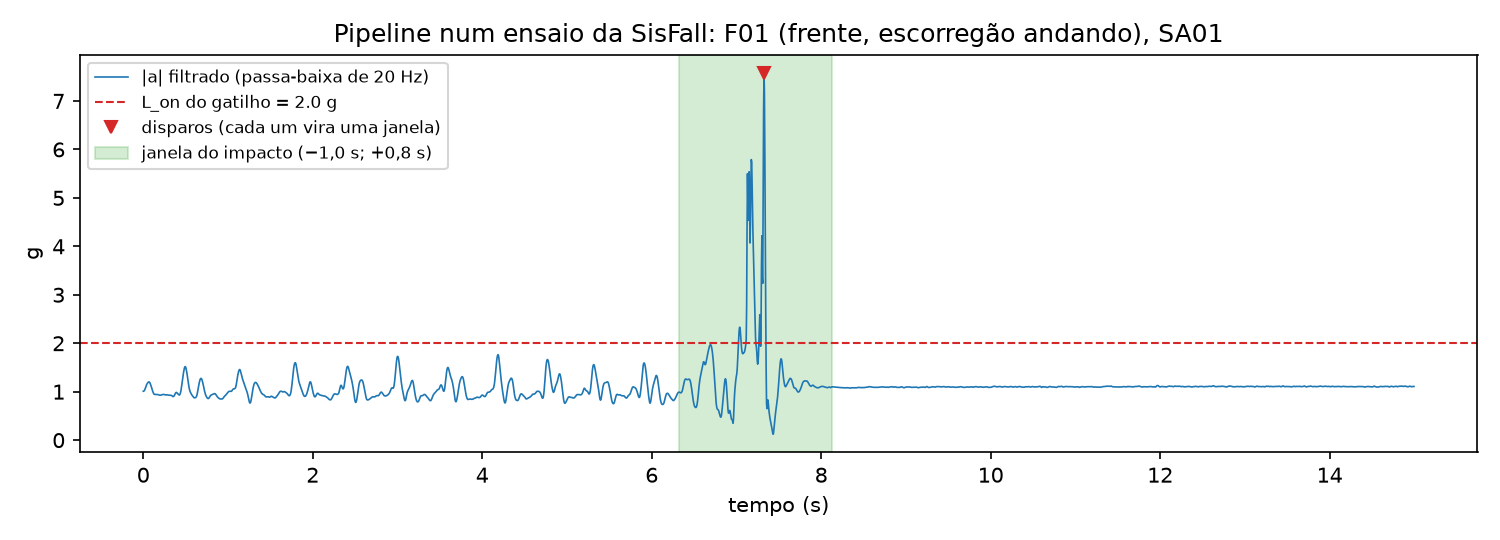
\includegraphics[width=\linewidth]{figuras/fig_pipeline.png}
  \caption{O pipeline numa queda da SisFall (F01, escorregão andando): $\amag$
  filtrado, limiar do gatilho, disparo e a janela que vai para o classificador.}
  \label{fig:pipeline}
\end{figure}

\paragraph{Por que detecção de picos, e não histerese.} A primeira versão do gatilho
usava a histerese do firmware, com período refratário. Ela escondia o impacto atrás de
um disparo da caminhada que precede a queda, e só cerca de 93\,\% das quedas
passavam; baixar o limiar piorava. Com o detector de picos, o maior pico do ensaio (o
impacto) sempre gera uma janela. Um teste automático cobre esse caso
(Seção~\ref{sec:testes}).

\paragraph{Escolha de $L_\text{on}$.} A Tabela~\ref{tab:gatilho} e a
Figura~\ref{fig:gatilho} mostram a varredura. Escolhemos o maior limiar que ainda
deixa passar pelo menos 99\,\% das quedas: \textbf{2,0\,g}, com 99,2\,\% das quedas e
858 disparos por hora de atividade no cenário A (862 no B). Nos nossos ensaios, passam
todas as quedas.

\begin{table}[H]
\centering
\caption{Varredura do limiar $L_\text{on}$ do gatilho no cenário A (SisFall): fração das quedas cujo impacto dispara o gatilho e disparos por hora de atividade, que viram janelas para o classificador. Escolhido: 2,0\,g.}
\label{tab:gatilho}
\small
\setlength{\tabcolsep}{4pt}
\begin{tabular}{ccc}
\toprule
$L_\text{on}$ (g) & Quedas que passam & Disparos por hora \\
\midrule
\num{1.50} & \num{100.0}\,\% & \num{1571} \\
\num{1.75} & \num{99.8}\,\% & \num{1090} \\
\num{2.00} & \num{99.2}\,\% & \num{858} \\
\num{2.25} & \num{98.1}\,\% & \num{730} \\
\num{2.50} & \num{97.0}\,\% & \num{636} \\
\num{2.75} & \num{95.2}\,\% & \num{545} \\
\num{3.00} & \num{92.2}\,\% & \num{449} \\
\num{3.25} & \num{89.7}\,\% & \num{354} \\
\num{3.50} & \num{86.5}\,\% & \num{269} \\
\num{3.75} & \num{82.0}\,\% & \num{199} \\
\num{4.00} & \num{77.1}\,\% & \num{146} \\
\bottomrule
\end{tabular}
\end{table}


\begin{figure}[H]
  \centering
  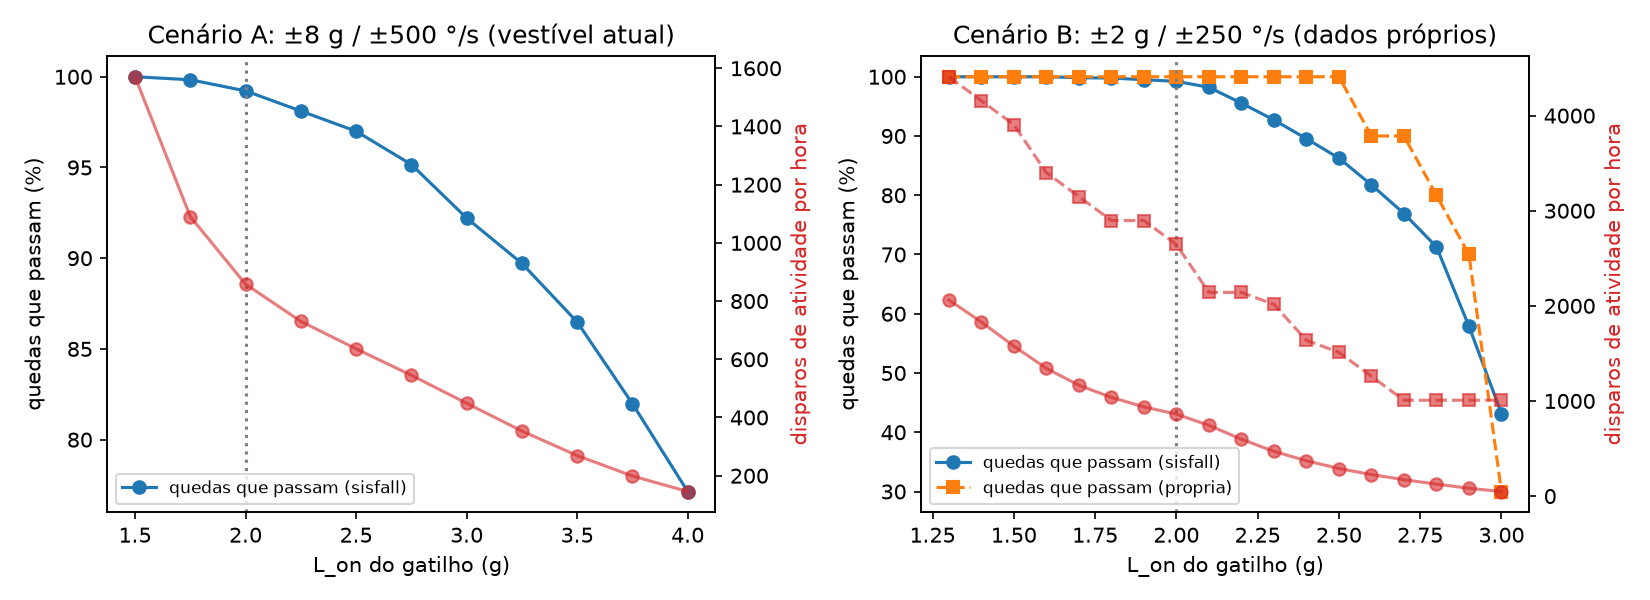
\includegraphics[width=\linewidth]{figuras/fig_gatilho.png}
  \caption{Varredura de $L_\text{on}$: quedas cujo impacto passa pelo gatilho (azul,
  eixo da esquerda) e disparos por hora de atividade (vermelho, eixo da direita). No
  cenário B, as linhas laranja são os nossos ensaios. A linha pontilhada marca 2,0\,g.}
  \label{fig:gatilho}
\end{figure}

A Figura~\ref{fig:funil} resume o papel de cada etapa: o gatilho deixa passar 1784 das
1798 quedas e acorda o classificador cerca de 858 vezes por hora; o classificador
mantém 1695 quedas e reduz os alarmes a 0,4 por hora.

\begin{figure}[H]
  \centering
  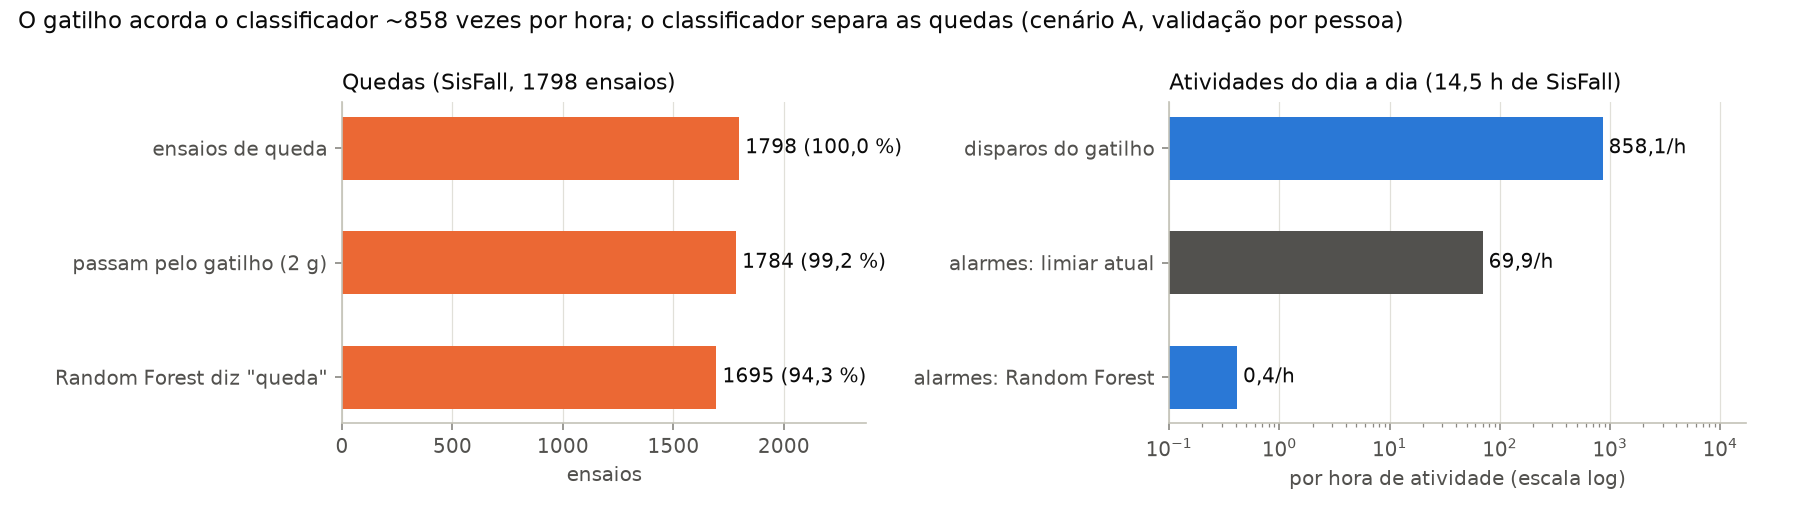
\includegraphics[width=\linewidth]{figuras/fig_funil.png}
  \caption{O que cada etapa deixa passar no cenário A, com o Random Forest como
  classificador. À esquerda, quedas (ensaios); à direita, atividades (por hora, em
  escala log), comparando os alarmes do limiar atual com os do Random Forest.}
  \label{fig:funil}
\end{figure}

\paragraph{Rótulos.} De cada ensaio de queda entra \textbf{uma} janela positiva: a do
disparo mais perto do maior $\amag$ do ensaio (até 0,5\,s). Os outros disparos do mesmo
ensaio, como os passos antes de escorregar, são ambíguos e ficam de fora. De cada
atividade entram \textbf{todas} as janelas, negativas: cada uma classificada como queda
é um alarme falso. No cenário A são 14\,256 janelas, 1784 de quedas e 12\,472 de
atividades.

%======================================================================
\section{Modelos}\label{sec:modelos}
%======================================================================
Cada modelo devolve um \emph{escore} por janela, maior quanto mais parecida com queda;
o limiar sobre o escore sai da avaliação (Seção~\ref{sec:metricas}). A
Tabela~\ref{tab:metodos} resume os métodos, e as subseções detalham os das aulas.

\begin{table}[H]
\centering
\caption{Métodos comparados. ``Aula'': slides da disciplina \cite{slides}.}
\label{tab:metodos}
\small
\begin{tabular}{@{}>{\raggedright\arraybackslash}p{3.6cm}>{\raggedright\arraybackslash}p{9.0cm}l@{}}
\toprule
Método & Ideia & Fonte \\
\midrule
Correlação com templates & pico da correlação cruzada entre $\amag$ e 8 templates de cada classe; normalizada (só a forma) e não normalizada (depende da energia) & aula \\
DTW & distância DTW aos mesmos templates, com banda de Sakoe--Chiba & aula \\
AR e ARX como anomalia & AR($p$) ajustado só em atividades; escore = maior erro de predição; o ARX usa $\wmag$ como entrada & aula \\
Distâncias & centroide mais próximo e kNN sobre os atributos, com distância euclidiana, Manhattan e cosseno & aula \\
Regras em cascata & queda livre e, depois, corpo parado ou inclinado & literatura \\
Regressão logística, árvore, SVM, Random Forest & classificadores sobre o vetor de atributos (tempo, FFT e AR) & literatura \\
CNN 1D & rede convolucional sobre a janela; aprende os próprios filtros & literatura \\
\bottomrule
\end{tabular}
\end{table}

\subsection{Correlação cruzada com templates}
Seja $x[n]$ a janela ($\amag$ a 50\,Hz, $N=90$) e $r[n]$ um template. A correlação
\textbf{normalizada} no atraso $m$ é o coeficiente de Pearson na parte sobreposta,
\begin{equation}\label{eq:corr_norm}
  \rho_{xr}[m]=\frac{\sum_n\bigl(x[n+m]-\bar x\bigr)\bigl(r[n]-\bar r\bigr)}
  {\sqrt{\sum_n\bigl(x[n+m]-\bar x\bigr)^2\,\sum_n\bigl(r[n]-\bar r\bigr)^2}}\in[-1,1],
\end{equation}
e a \textbf{não normalizada} é a média do produto, $c_{xr}[m]=\frac1{N'}\sum_n
x[n+m]\,r[n]$, que cresce com a energia da janela. Usamos atrasos de $\pm10$ amostras
($\pm0{,}2$\,s). Os templates são 8 medoides de cada classe, escolhidos nas dobras de
treino: \emph{k-means} sobre as janelas e, de cada grupo, a janela real mais perto do
centro. O escore compara as duas classes:
\begin{equation}\label{eq:escore_templates}
  s(x)=\max_{k,m}\rho\bigl(x,r^{\text{queda}}_k\bigr)[m]-\max_{k,m}\rho\bigl(x,r^{\text{ativ.}}_k\bigr)[m].
\end{equation}

\subsection{DTW}
A DTW alinha $r$ ($N$ amostras) e $x$ ($M$ amostras) deformando o tempo. Com custo
$|r_i-x_j|$, a distância acumulada é
\begin{equation}\label{eq:dtw}
  D(i,j)=|r_i-x_j|+\min\bigl\{D(i-1,j),\,D(i,j-1),\,D(i-1,j-1)\bigr\},
\end{equation}
calculada só na banda de Sakoe--Chiba $|i-jN/M|\le9$ \cite{sakoe}, e a distância é
$D(N,M)$. O escore é o da Eq.~\eqref{eq:escore_templates}, com a menor distância no
lugar da maior correlação (e o sinal trocado).

\subsection{Modelos autorregressivos AR e ARX}\label{sec:ar}
O modelo AR($p$) prevê cada amostra pelas $p$ anteriores \cite{box}:
\begin{equation}\label{eq:ar}
  x[n]=c+\sum_{k=1}^{p}a_k\,x[n-k]+e[n].
\end{equation}
Empilhando as equações de todas as amostras, $\mathbf b=\mathbf A\boldsymbol\theta+\mathbf e$,
com $\boldsymbol\theta=[c,a_1,\dots,a_p]^\mathsf T$, os coeficientes saem por mínimos
quadrados,
\begin{equation}\label{eq:mmq}
  \hat{\boldsymbol\theta}=\bigl(\mathbf A^\mathsf T\mathbf A\bigr)^{-1}\mathbf A^\mathsf T\mathbf b .
\end{equation}
O ARX($p$) acrescenta uma entrada exógena $u[n]$, aqui $\wmag$:
$x[n]=c+\sum_{k=1}^{p}a_kx[n-k]+\sum_{k=0}^{p}b_ku[n-k]+e[n]$. A ordem é escolhida pelos
critérios de informação \cite{akaike,schwarz}, com $N$ amostras e variância do resíduo
$\hat\sigma^2_e$:
\begin{equation}\label{eq:aic_bic}
  \text{AIC}=N\ln\hat\sigma^2_e+2p,\qquad \text{BIC}=N\ln\hat\sigma^2_e+p\ln N .
\end{equation}

O AR entra de duas formas:
\begin{itemize}[leftmargin=1.5em]
\item \textbf{detector de anomalia:} o AR($p$) é ajustado \emph{só nas janelas de
  atividade} do treino. Numa queda o modelo deveria errar muito; o escore é o maior erro
  de predição a um passo na janela, $s=\max_n|x[n]-\hat x[n]|$;
\item \textbf{atributos:} os coeficientes de um AR(4) ajustado em cada janela e o
  desvio do seu resíduo entram no vetor de atributos dos classificadores.
\end{itemize}

\subsection{Atributos}\label{sec:atributos}
Calculados sobre a janela de 200\,Hz:
\begin{itemize}[leftmargin=1.5em]
\item \textbf{no tempo:} média, RMS, desvio, mínimo, máximo e fator de crista de
  $\amag$ (as mesmas fórmulas do \code{signal\_proc.c} do vestível); curtose,
  assimetria, taxa de cruzamentos por zero e pico a pico de $\amag$; SMA; queda livre
  (mínimo de $\amag$ antes do impacto e tempo até o impacto); desvio e média de $\amag$
  nos últimos 0,3\,s (quietude); mudança de inclinação (ângulo entre a aceleração média
  no início e no fim); $|$correlação$|$ entre eixos; média, RMS e pico de $\wmag$ e
  rotação total;
\item \textbf{em frequência:} FFT de 512 pontos de $\amag$ sem a média e com janela de
  Hann: fração da energia nas bandas 0,5--3, 3--6, 6--12 e 12--25\,Hz, frequência
  dominante e centroide espectral;
\item \textbf{AR:} os 4 coeficientes de um AR(4) e o desvio do resíduo.
\end{itemize}
São 34 atributos no total.

\subsection{Distâncias e classificadores}
Sobre os atributos padronizados:
\begin{itemize}[leftmargin=1.5em]
\item \textbf{centroide mais próximo:} o escore é a distância ao centroide das
  atividades menos a distância ao centroide das quedas, com distância euclidiana,
  Manhattan ou cosseno;
\item \textbf{kNN:} $k=7$ vizinhos, ponderados pela distância, com as mesmas três
  distâncias;
\item \textbf{regressão logística}, \textbf{árvore de decisão} (profundidade 6),
  \textbf{SVM} com núcleo RBF ($C=3$; 6000 janelas de atividade sorteadas para o
  treino) e \textbf{Random Forest} \cite{breiman} (150 árvores, profundidade 12), todos
  com classes balanceadas \cite{sklearn};
\item \textbf{regras em cascata:} queda livre ($\amag<0{,}6$\,g antes do impacto) e,
  depois, corpo parado (desvio $<0{,}15$\,g) ou inclinação $>40$°;
\item \textbf{ablação:} o Random Forest só com cada grupo de atributos (tempo, FFT, AR).
\end{itemize}

\subsection{CNN 1D}
Uma rede convolucional \cite{pytorch} com três camadas (16 filtros de largura 7, 32 de
largura 5 e 32 de largura 3, com normalização em lote, ReLU e \emph{pooling}), média
global e uma saída. Cada camada é um banco de filtros FIR aprendidos: a rede aprende os
próprios templates. A entrada é a janela a 50\,Hz, só com os módulos ($\amag$, $\wmag$)
ou com os 6 eixos. Treino: Adam, taxa $10^{-3}$, 15 épocas, lotes de 256 e perda
ponderada pela proporção das classes.

%======================================================================
\section{Avaliação e testes}\label{sec:avaliacao}
%======================================================================
\subsection{Validação cruzada por pessoa}
A SisFall tem várias repetições de cada movimento por pessoa. Se janelas da mesma
pessoa ficassem no treino e no teste, o modelo reconheceria a pessoa, e não a queda,
e os resultados ficariam inflados. Por isso a validação cruzada é \textbf{por pessoa}
(\code{StratifiedGroupKFold}, 5 dobras): cada janela recebe o escore de um modelo
treinado sem nenhuma janela da sua pessoa. O programa confere, em cada dobra, que
nenhuma pessoa aparece no treino e no teste. Templates, centroides, AR e normalizações
são calculados só nas dobras de treino.

\subsection{Métricas}\label{sec:metricas}
\begin{itemize}[leftmargin=1.5em]
\item \textbf{AUC} da curva ROC por janela.
\item \textbf{Ponto de operação:} o limiar que deixa 95\,\% das janelas de impacto
  acima dele. Nesse ponto:
  \begin{itemize}
  \item \textbf{quedas detectadas}, por ensaio, contando também as que o gatilho perdeu;
  \item \textbf{alarmes falsos por hora} de atividade (14,5\,h na SisFall).
  \end{itemize}
\item \textbf{Quedas detectadas com no máximo 1 alarme falso por hora}: a métrica mais
  próxima do uso real.
\item \textbf{Custo estimado no ESP32-S3:} operações por janela (com os atributos) e
  tamanho do modelo.
\end{itemize}
\textbf{Linha de base:} o detector atual do firmware, reimplementado (histerese em
$\amag^2$ com 6,25 e 2,25\,g$^2$, evento de até 1\,s, espera de 30\,s), decidindo
sozinho.

\subsection{Testes automáticos e verificações}\label{sec:testes}
Os blocos do pipeline são testados contra valores conhecidos e contra os exemplos
numéricos dos slides. Os 13 testes passam (\code{pytest}); a
Tabela~\ref{tab:testes} mostra o que cada um confere.

\begin{table}[H]
\centering
\caption{Testes automáticos de \code{modelo/tests/test\_blocos.py}.}
\label{tab:testes}
\small
\begin{tabular}{@{}>{\raggedright\arraybackslash}p{5.2cm}>{\raggedright\arraybackslash}p{10.2cm}@{}}
\toprule
Bloco & O que o teste confere \\
\midrule
AR por mínimos quadrados & $x=[2,3,4,5,6,7]$ dá $a_1=2$ e $a_2=-1$ com resíduo nulo, como no slide \\
DTW & $r=[1,3,1]$ e $x=[1,1,3,3,1]$ têm distância 0, como no slide; sinais diferentes têm distância positiva (2 testes) \\
Correlação normalizada & um sinal consigo mesmo dá 1; multiplicar por 5 não muda a normalizada e multiplica a não normalizada por 5 \\
Atributos no tempo & RMS $=1/\sqrt2$ e fator de crista $=\sqrt2$ num seno (as fórmulas do \code{signal\_proc.c}); curtose da normal $\approx3$; 20 cruzamentos por zero num seno de 5\,Hz em 2\,s (3 testes) \\
FFT & acha a frequência dominante de um seno \\
Histerese do firmware & um pico por evento; respeita o período refratário (2 testes) \\
Gatilho & o impacto não fica escondido atrás de um disparo anterior; a versão vetorizada é igual ao laço amostra a amostra do firmware em 50 sinais aleatórios (2 testes) \\
Janela & no fim do ensaio, a última amostra é repetida \\
\bottomrule
\end{tabular}
\end{table}

Além dos testes, o programa faz verificações a cada execução:
\begin{itemize}[leftmargin=1.5em]
\item nenhuma pessoa no treino e no teste da mesma dobra;
\item os escores salvos correspondem às janelas recalculadas;
\item o Random Forest retreinado para as figuras dá, arquivo a arquivo, o mesmo
  resultado da tabela dos nossos ensaios;
\item rodar de novo a comparação do cenário A reproduz todos os números.
\end{itemize}
Nada disso roda ainda no ESP32: esta entrega é toda no computador.

%======================================================================
\section{Resultados}\label{sec:resultados}
%======================================================================
\subsection{Comparação geral}
A Tabela~\ref{tab:comparacao_A} traz todos os métodos no cenário A, e a
Figura~\ref{fig:resumo}, os principais nos dois cenários.

\begin{table}[H]
\centering
\caption{Comparação dos métodos no cenário A ($\pm$8\,g, vestível atual), SisFall com validação cruzada por pessoa (5 dobras). ``Quedas'' e ``alarmes/h'': no ponto em que 95\,\% das janelas de impacto ficam acima do limiar; as quedas são contadas por ensaio, inclusive as que o gatilho perdeu. ``Quedas com $\le$1 alarme/h'': maior fração de quedas detectadas com no máximo um alarme falso por hora de atividade. Custo no ESP32-S3: milhares de operações por janela (com os atributos) e tamanho do modelo, ambos estimados.}
\label{tab:comparacao_A}
\footnotesize
\setlength{\tabcolsep}{4pt}
\begin{tabular}{@{}llcccccr@{}}
\toprule
Método & Família & AUC & Quedas & \makecell{Alarmes\\por hora} & \makecell{Quedas com\\$\le$1 alarme/h} & \makecell{Operações\\($\times10^3$)} & Modelo \\
\midrule
Limiar atual (2,5\,g) & base & --- & \num{97.4}\,\% & \num{69.9} & --- & --- & \num{8}\,B \\
\midrule
Regras em cascata & lit. & \num{0.977} & \num{94.3}\,\% & \num{54.9} & \num{23.5}\,\% & \num{44.7} & \num{12}\,B \\
\midrule
Correlação não normalizada & aula & \num{0.957} & \num{94.3}\,\% & \num{139.2} & \num{22.0}\,\% & \num{30.2} & \num{5.8}\,kB \\
Correlação normalizada & aula & \num{0.956} & \num{94.3}\,\% & \num{90.9} & \num{1.3}\,\% & \num{30.2} & \num{5.8}\,kB \\
DTW & aula & \num{0.974} & \num{94.3}\,\% & \num{74.0} & \num{7.6}\,\% & \num{27.4} & \num{5.8}\,kB \\
AR(12) como anomalia & aula & \num{0.786} & \num{94.3}\,\% & \num{688.1} & \num{8.6}\,\% & \num{1.2} & \num{52}\,B \\
ARX(12) como anomalia & aula & \num{0.789} & \num{94.3}\,\% & \num{676.4} & \num{11.4}\,\% & \num{2.3} & \num{104}\,B \\
Centroide (euclidiana) & aula & \num{0.993} & \num{94.3}\,\% & \num{23.1} & \num{51.1}\,\% & \num{44.8} & \num{544}\,B \\
Centroide (Manhattan) & aula & \num{0.992} & \num{94.3}\,\% & \num{28.5} & \num{44.2}\,\% & \num{44.8} & \num{544}\,B \\
Centroide (cosseno) & aula & \num{0.996} & \num{94.3}\,\% & \num{15.8} & \num{62.3}\,\% & \num{44.8} & \num{544}\,B \\
kNN (euclidiana) & aula & \num{0.996} & \num{94.3}\,\% & \num{0.8} & \num{94.9}\,\% & \num{820.0} & \num{1.55}\,MB \\
kNN (Manhattan) & aula & \num{0.995} & \num{94.3}\,\% & \num{0.5} & \num{96.1}\,\% & \num{820.0} & \num{1.55}\,MB \\
kNN (cosseno) & aula & \num{0.995} & \num{94.3}\,\% & \num{1.6} & \num{93.3}\,\% & \num{820.0} & \num{1.55}\,MB \\
\midrule
Regressão logística & lit. & \num{0.997} & \num{94.3}\,\% & \num{1.4} & \num{92.8}\,\% & \num{44.8} & \num{412}\,B \\
Árvore de decisão & lit. & \num{0.986} & \num{95.9}\,\% & \num{5.3} & \num{0.0}\,\% & \num{44.7} & \num{612}\,B \\
SVM (RBF) & lit. & \num{0.998} & \num{94.3}\,\% & \num{0.8} & \num{94.6}\,\% & \num{77.8} & \num{45.4}\,kB \\
\midrule
RF: só tempo & ablação & \num{0.999} & \num{94.3}\,\% & \num{0.8} & \num{95.4}\,\% & \num{16.2} & \num{240.1}\,kB \\
RF: só FFT & ablação & \num{0.927} & \num{94.3}\,\% & \num{274.4} & \num{7.8}\,\% & \num{24.8} & \num{1.34}\,MB \\
RF: só AR(4) & ablação & \num{0.706} & \num{94.3}\,\% & \num{706.8} & \num{5.2}\,\% & \num{9.1} & \num{1.39}\,MB \\
RF: tempo + FFT & ablação & \num{0.999} & \num{94.3}\,\% & \num{0.5} & \num{95.5}\,\% & \num{39.2} & \num{236.6}\,kB \\
\midrule
\textbf{Random Forest} & lit. & \num{0.999} & \num{94.3}\,\% & \num{0.4} & \num{95.7}\,\% & \num{46.5} & \num{251.7}\,kB \\
CNN 1D (módulos) & lit. & \num{0.994} & \num{94.3}\,\% & \num{17.2} & \num{59.1}\,\% & \num{203.0} & \num{24.3}\,kB \\
CNN 1D (6 eixos) & lit. & \num{0.998} & \num{94.3}\,\% & \num{1.2} & \num{93.9}\,\% & \num{243.3} & \num{26.1}\,kB \\
\bottomrule
\end{tabular}
\end{table}


\begin{figure}[H]
  \centering
  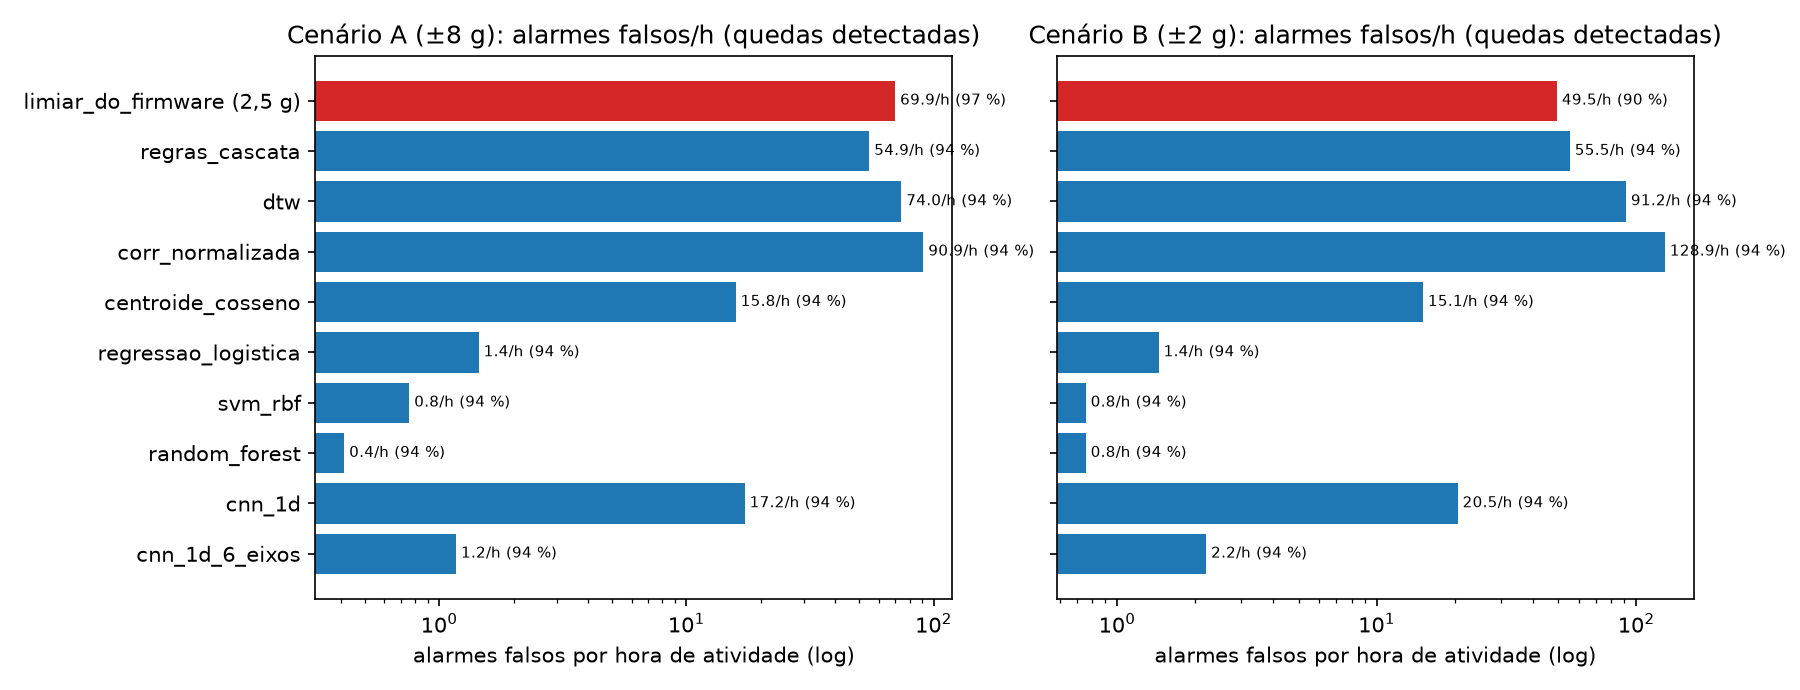
\includegraphics[width=\linewidth]{figuras/fig_resumo.png}
  \caption{Alarmes falsos por hora de atividade (escala log) no ponto de operação, com
  a fração das quedas detectadas entre parênteses. Vermelho: o limiar atual do
  firmware.}
  \label{fig:resumo}
\end{figure}

Com praticamente a mesma sensibilidade (94,3\,\% das quedas), os alarmes falsos vão de
69,9 por hora no limiar atual e 74 a 139 nos métodos de comparar formas (correlação e
DTW) para 0,4 no Random Forest, 0,8 no SVM e 1,4 na regressão logística. A
Figura~\ref{fig:escores} mostra por quê: nos métodos de atributos, as distribuições dos
escores de quedas e de atividades quase não se sobrepõem. A Figura~\ref{fig:roc} mostra
as curvas ROC.

\begin{figure}[H]
  \centering
  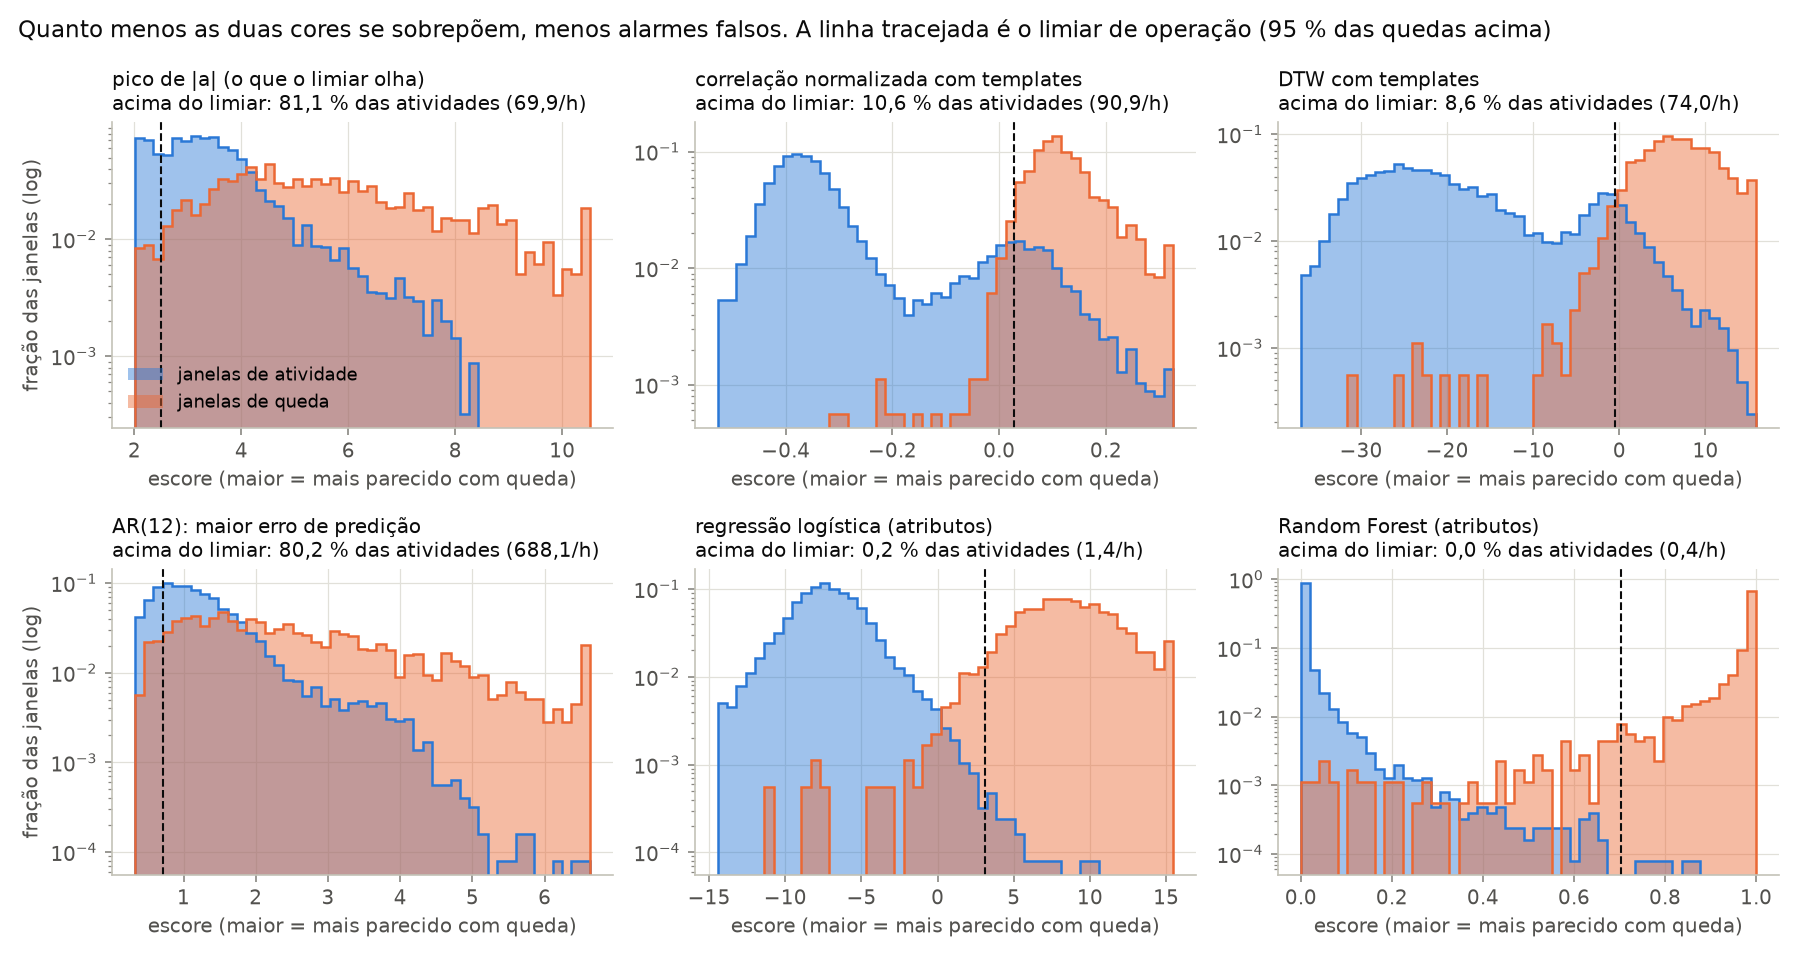
\includegraphics[width=\linewidth]{figuras/fig_escores.png}
  \caption{Distribuição dos escores das janelas de queda (laranja) e de atividade
  (azul), cada classe normalizada para somar 1, em escala log, em seis métodos. A
  linha tracejada é o limiar de operação; acima dela, a fração das atividades que vira
  alarme falso.}
  \label{fig:escores}
\end{figure}

\begin{figure}[H]
  \centering
  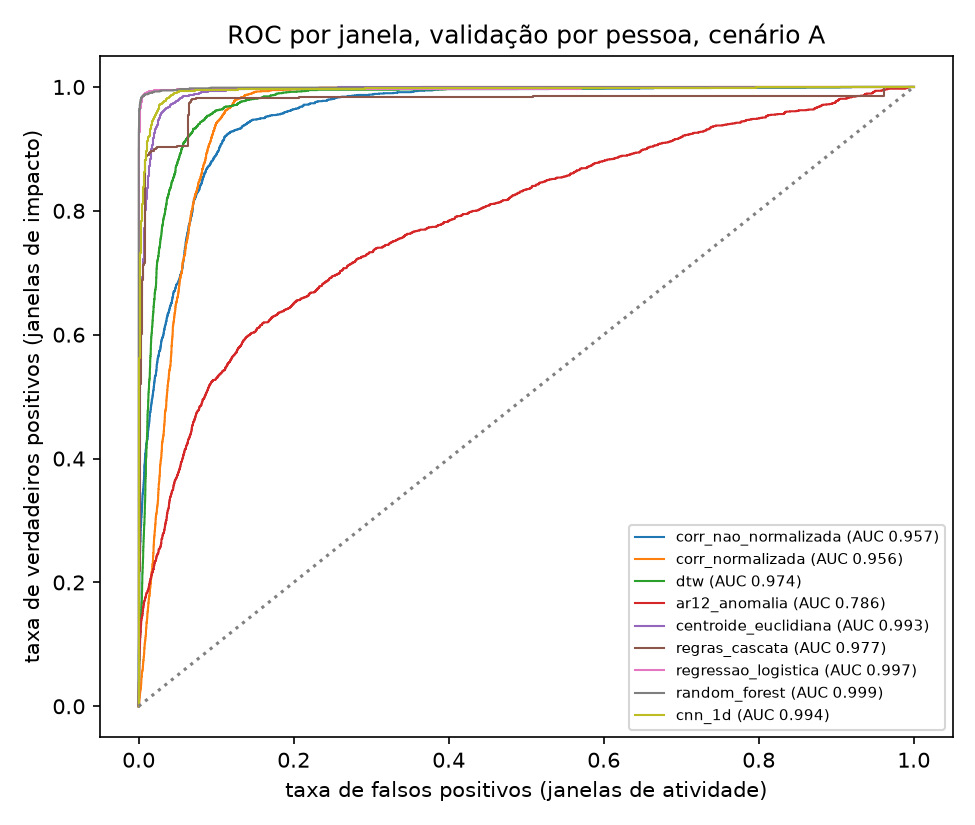
\includegraphics[width=0.72\linewidth]{figuras/fig_roc_A.png}
  \caption{Curvas ROC por janela no cenário A, com validação por pessoa.}
  \label{fig:roc}
\end{figure}

\subsection{O que separa a queda de uma corrida}
O pico de $\amag$ sozinho não separa: correr, subir escada rápido, tropeçar e pular
passam de 2,5\,g como as quedas (Figura~\ref{fig:picos}). O que separa é o que vem
antes e depois do impacto (Figura~\ref{fig:separacao}): na queda, o corpo fica parado
(baixo desvio de $\amag$ no fim da janela) e deitado (grande mudança de inclinação).

\begin{figure}[H]
  \centering
  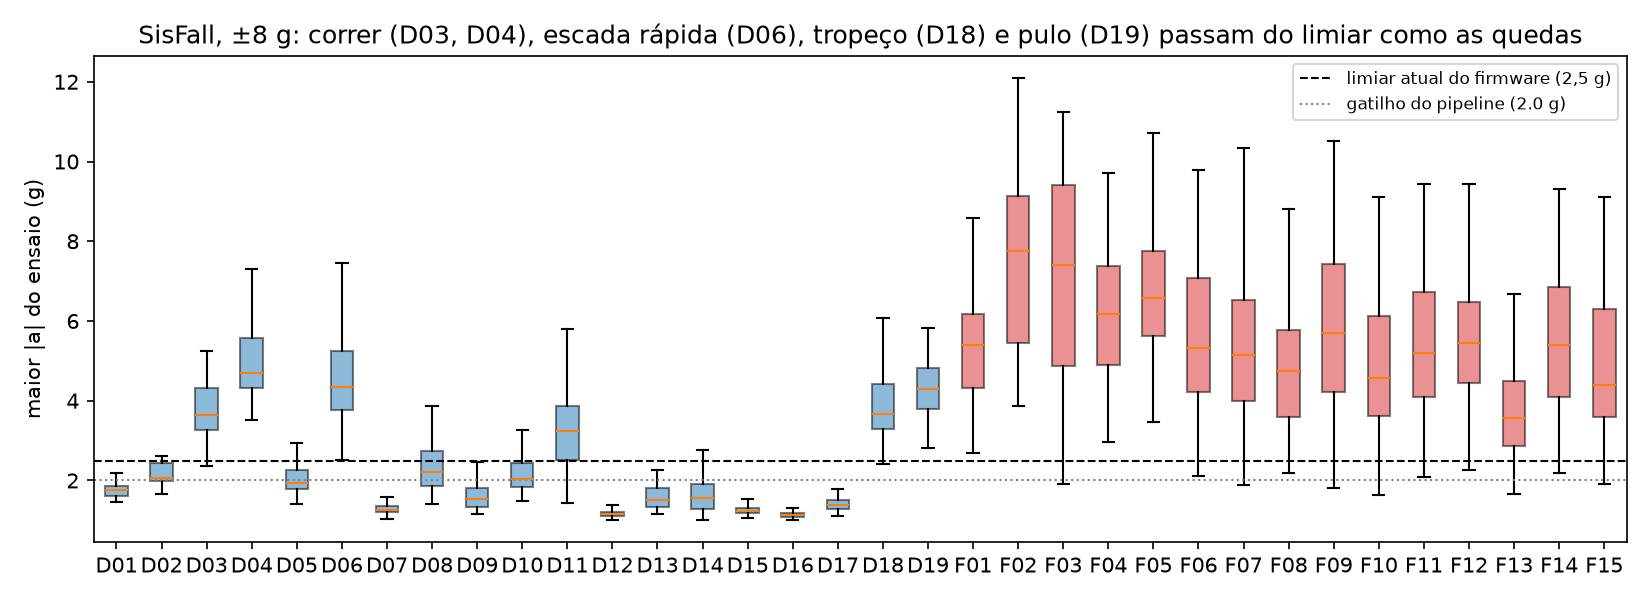
\includegraphics[width=\linewidth]{figuras/fig_picos.png}
  \caption{Maior $\amag$ de cada ensaio da SisFall ($\pm$8\,g), por tipo de atividade
  (azul) e de queda (vermelho). A linha tracejada é o limiar atual (2,5\,g); a
  pontilhada, o gatilho (2,0\,g).}
  \label{fig:picos}
\end{figure}

\begin{figure}[H]
  \centering
  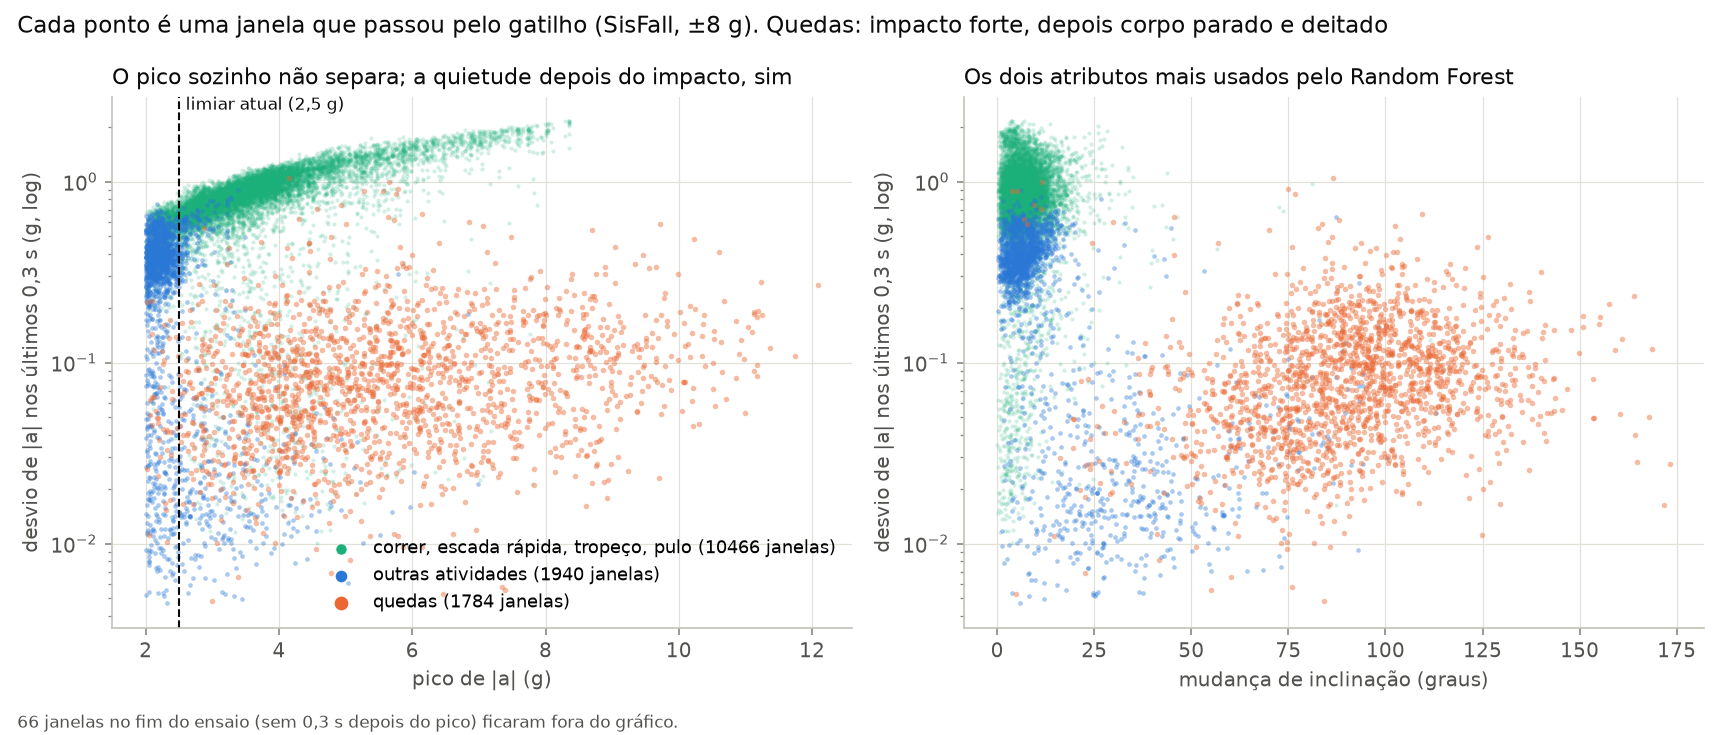
\includegraphics[width=\linewidth]{figuras/fig_separacao.png}
  \caption{Cada ponto é uma janela que passou pelo gatilho. À esquerda, pico de $\amag$
  $\times$ desvio de $\amag$ nos últimos 0,3\,s; à direita, os dois atributos mais
  usados pelo Random Forest. Verde: correr, escada rápida, tropeço e pulo.}
  \label{fig:separacao}
\end{figure}

A importância dos atributos no Random Forest e a ablação por grupo
(Figura~\ref{fig:atributos}) confirmam: os atributos mais usados são a mudança de
inclinação (25,5\,\% da importância), o desvio no fim da janela (16,2\,\%) e a curtose
de $\amag$ (13,8\,\%). Com 1 alarme falso por hora no máximo, só os atributos no tempo
detectam 95,4\,\% das quedas; só os de FFT, 7,8\,\%; só os do AR(4), 5,2\,\%; todos
juntos, 95,7\,\%.

\begin{figure}[H]
  \centering
  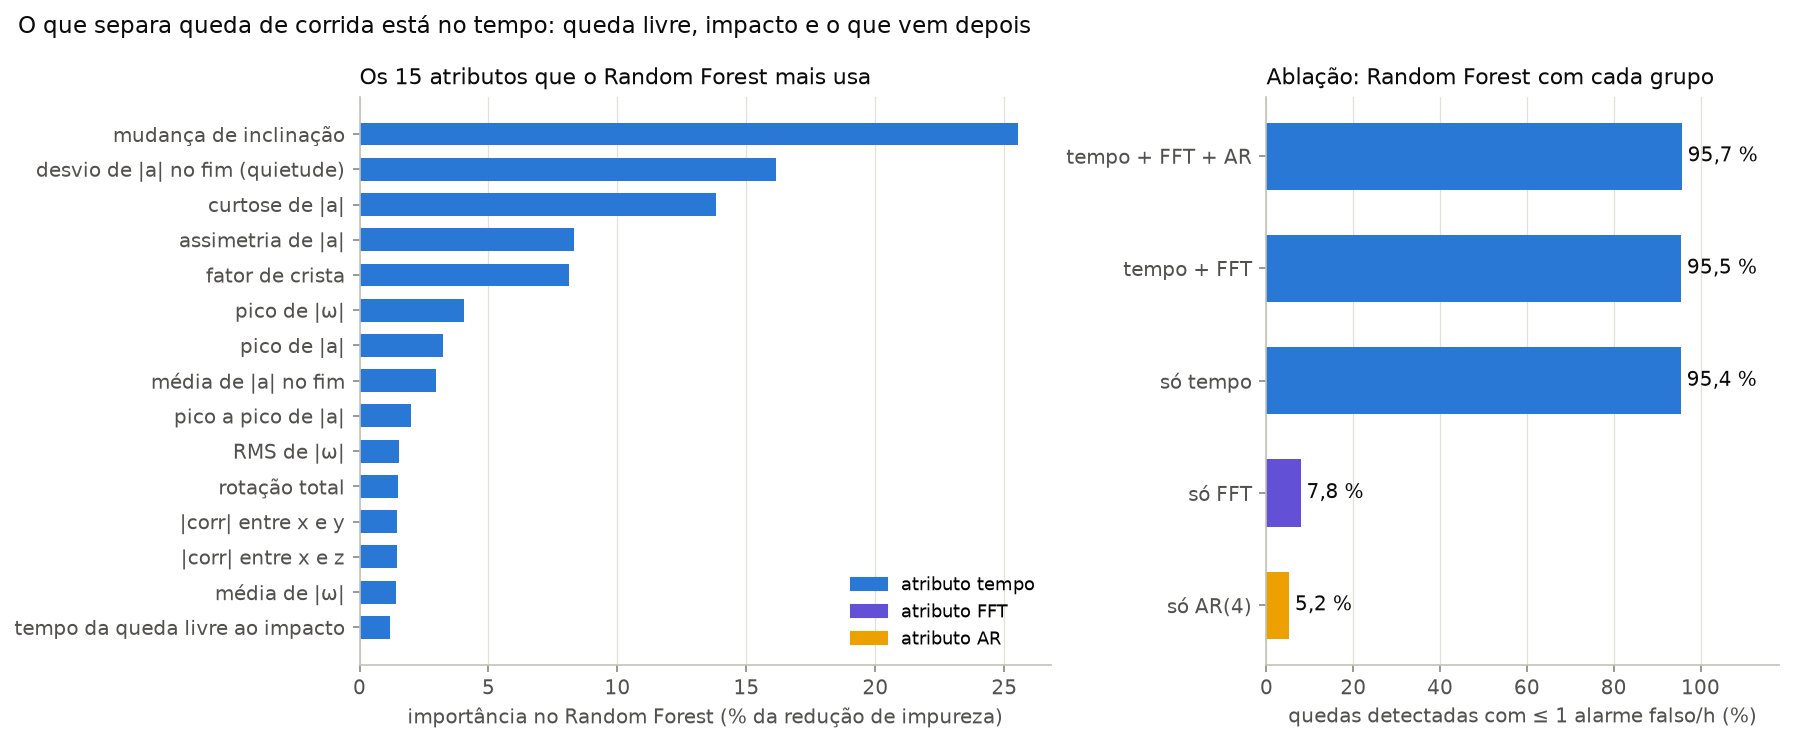
\includegraphics[width=\linewidth]{figuras/fig_atributos_rf.png}
  \caption{À esquerda, os 15 atributos mais importantes no Random Forest treinado em
  toda a SisFall (cenário A). À direita, a ablação: Random Forest com cada grupo de
  atributos, quedas detectadas com $\le$1 alarme falso por hora.}
  \label{fig:atributos}
\end{figure}

A FFT separa bem andar de correr, mas não a corrida da queda
(Figura~\ref{fig:fft}): a corrida concentra energia em 2--3\,Hz e a queda é mais
espalhada, mas as distribuições se sobrepõem, e a janela de 1,8\,s tem resolução
espectral de só cerca de 0,55\,Hz.

\begin{figure}[H]
  \centering
  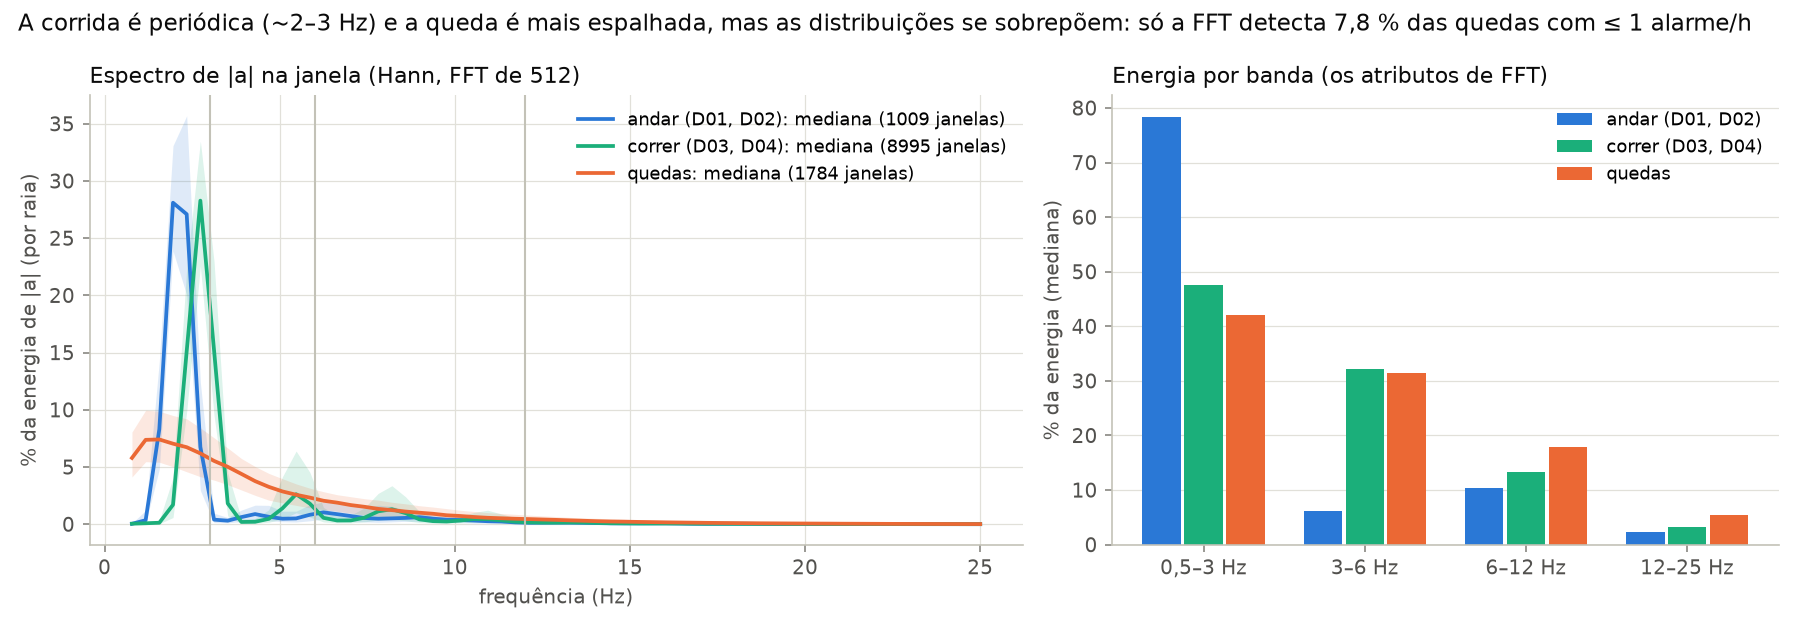
\includegraphics[width=\linewidth]{figuras/fig_fft.png}
  \caption{Espectro de $\amag$ na janela (mediana e faixa interquartil) ao andar,
  correr e cair, e a energia por banda usada como atributo.}
  \label{fig:fft}
\end{figure}

\subsection{Modelo autorregressivo}
A Tabela~\ref{tab:ordem_ar} e a Figura~\ref{fig:ordem_ar} mostram a escolha da ordem.
A variância do resíduo cai de 0,268\,g$^2$ em AR(1) para 0,194 em AR(2) e 0,114 em
AR(12), e o BIC continua caindo até $p=12$, a ordem usada no detector de anomalia.

\begin{table}[H]
\centering
\caption{Escolha da ordem do AR($p$) em $|a|$ a 50\,Hz, ajustado por mínimos quadrados em todas as janelas de atividade do cenário A: variância do resíduo e AIC e BIC em relação a $p=1$ (em milhares). O BIC continua caindo até $p=12$, o maior valor testado.}
\label{tab:ordem_ar}
\small
\setlength{\tabcolsep}{4pt}
\begin{tabular}{cccc}
\toprule
$p$ & $\sigma^2_e$ (g$^2$) & $\Delta$AIC ($\times10^3$) & $\Delta$BIC ($\times10^3$) \\
\midrule
1 & \num{0.268} & \num{0.0} & \num{0.0} \\
2 & \num{0.194} & \num{-339.0} & \num{-339.0} \\
3 & \num{0.186} & \num{-364.8} & \num{-364.8} \\
4 & \num{0.175} & \num{-406.1} & \num{-406.1} \\
5 & \num{0.170} & \num{-419.3} & \num{-419.2} \\
6 & \num{0.161} & \num{-455.4} & \num{-455.3} \\
7 & \num{0.154} & \num{-476.2} & \num{-476.2} \\
8 & \num{0.146} & \num{-508.4} & \num{-508.3} \\
9 & \num{0.138} & \num{-537.6} & \num{-537.5} \\
10 & \num{0.131} & \num{-569.8} & \num{-569.7} \\
11 & \num{0.123} & \num{-603.5} & \num{-603.3} \\
12 & \num{0.114} & \num{-652.1} & \num{-652.0} \\
\bottomrule
\end{tabular}
\end{table}


\begin{figure}[H]
  \centering
  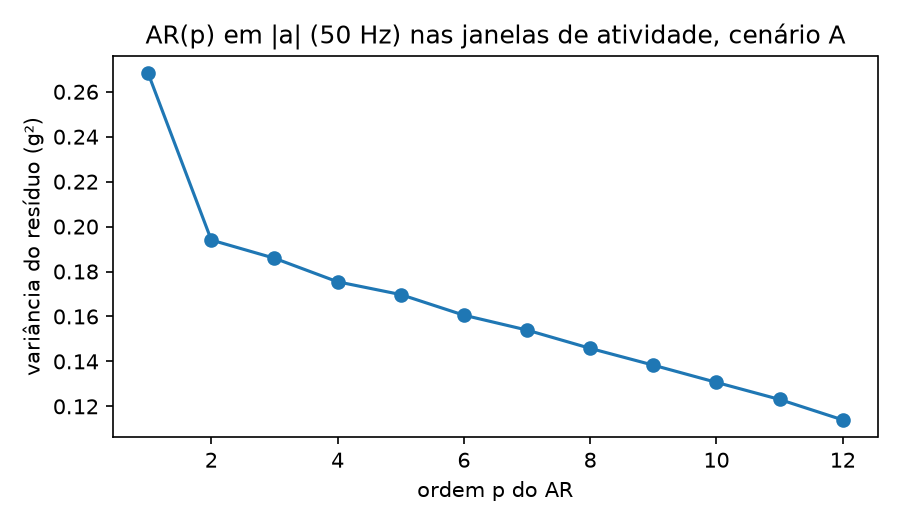
\includegraphics[width=0.62\linewidth]{figuras/fig_ordem_ar_A.png}
  \caption{Variância do resíduo do AR($p$) em $\amag$ (50\,Hz) nas janelas de
  atividade do cenário A.}
  \label{fig:ordem_ar}
\end{figure}

O AR descreve bem a atividade normal, mas, como detector de anomalia, é o pior método
(AUC 0,786; 688 alarmes falsos por hora). A Figura~\ref{fig:ar} mostra o motivo: o
modelo treinado em atividades erra no impacto da queda, mas também em cada passo de
corrida, que é um pico rápido que ele não consegue prever. O ARX, com $\wmag$ como
entrada, quase não muda (AUC 0,789).

\begin{figure}[H]
  \centering
  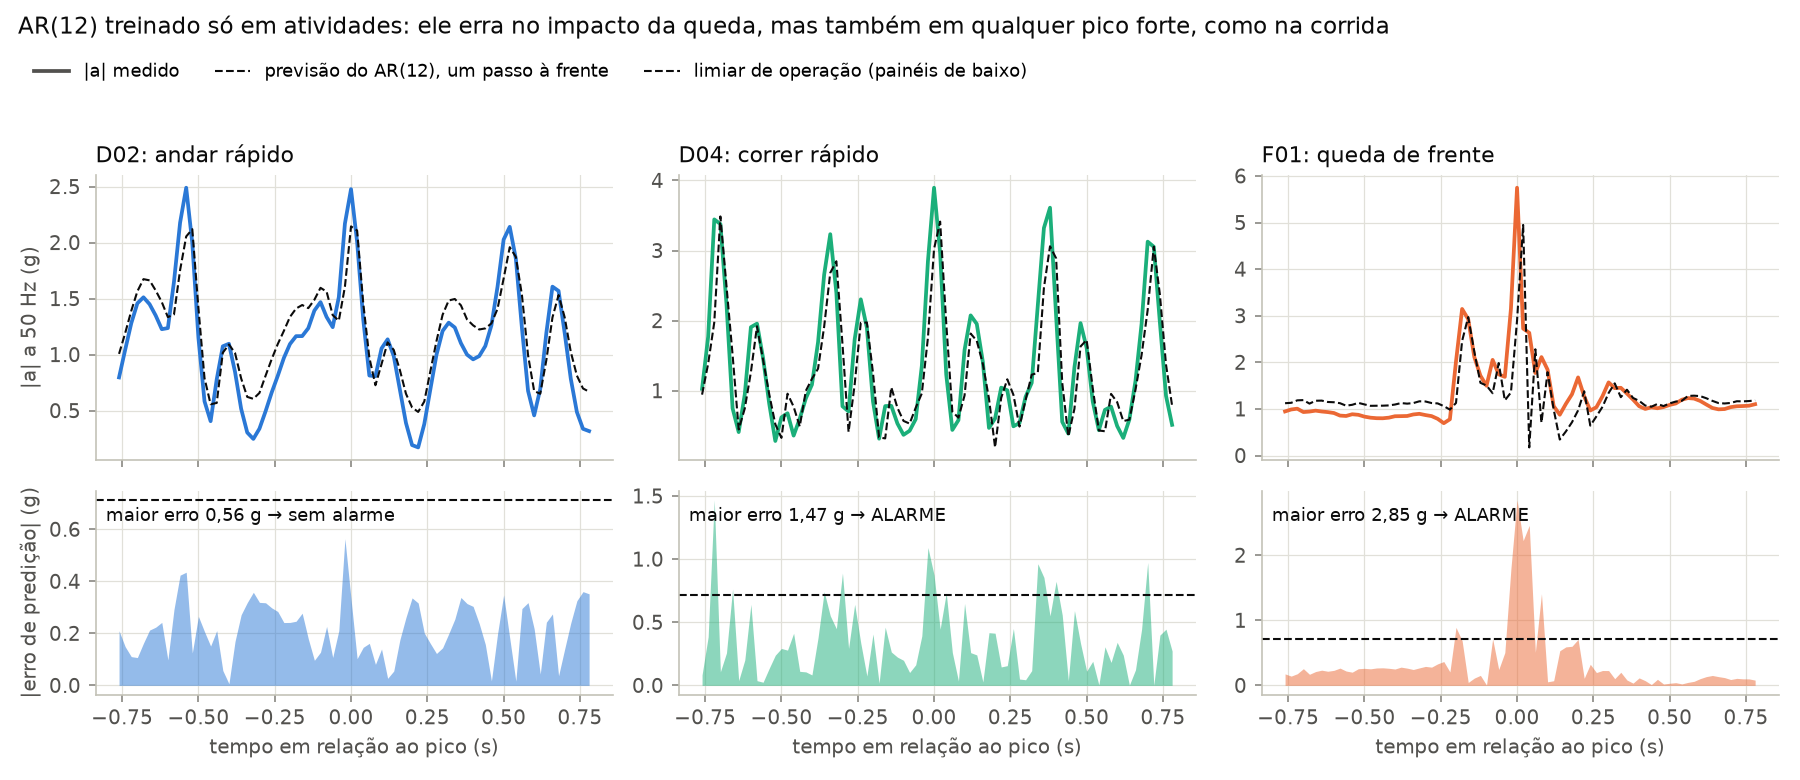
\includegraphics[width=\linewidth]{figuras/fig_ar_explicado.png}
  \caption{AR(12) treinado só em atividades, em janelas típicas (escore mediano do
  tipo) de andar rápido, correr rápido e uma queda de frente. Acima, $\amag$ e a
  previsão a um passo; abaixo, o erro de predição e o limiar de operação.}
  \label{fig:ar}
\end{figure}

\subsection{Correlação com templates e DTW}
A Figura~\ref{fig:templates} mostra os templates e dois exemplos. Os templates de
atividade são, na maioria, passos de corrida, que dominam as janelas (correr gera
muitos disparos). A queda típica casa muito bem com um template de queda ($\rho=0{,}95$),
mas também bastante com os de atividade (0,85), porque o pico do impacto domina a forma.
A corrida que dá alarme não se parece muito com queda ($\rho=0{,}44$), mas se parece
ainda menos com os templates de atividade (0,34); como o escore é a diferença, ela
passa do limiar. Comparar só a forma de $\amag$ não basta.

\begin{figure}[H]
  \centering
  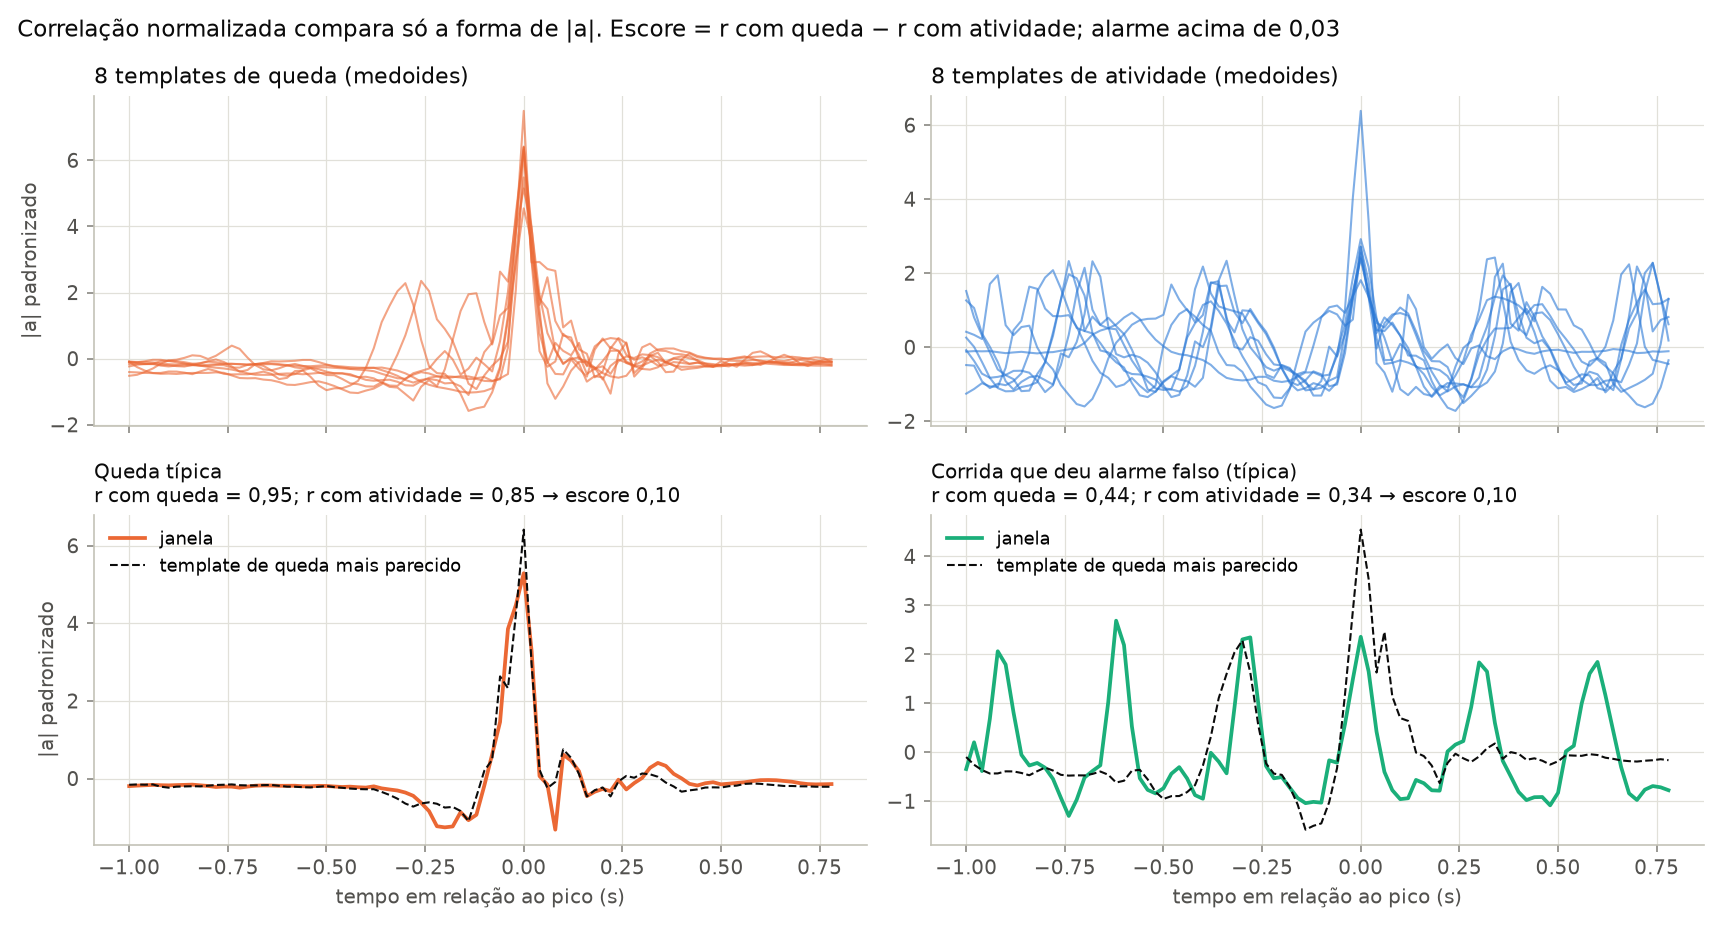
\includegraphics[width=\linewidth]{figuras/fig_templates.png}
  \caption{Correlação normalizada (cenário A). Acima, os 8 templates de cada classe,
  padronizados. Abaixo, uma queda típica e uma corrida típica entre as que deram alarme
  falso, cada uma com o template de queda mais parecido.}
  \label{fig:templates}
\end{figure}

\paragraph{Normalizada ou não normalizada?} No ponto de 95\,\% das quedas, a
normalizada dá menos alarmes (90,9 contra 139,2 por hora), porque compara só a forma.
Com poucos alarmes permitidos, a não normalizada vai melhor (22,0\,\% contra 1,3\,\% das
quedas com $\le$1 alarme por hora), porque a energia do impacto também informa. Quando o
sensor satura, essa energia some, e a não normalizada desaba: AUC de 0,957 para 0,843
(Tabela~\ref{tab:cenarios_AB}).

\subsection{Efeito da faixa do sensor}
A Tabela~\ref{tab:cenarios_AB} compara os dois cenários. Os métodos de atributos quase
não perdem com a saturação (Random Forest: 95,7\,\% para 94,4\,\% das quedas com $\le$1
alarme por hora), porque a postura e a quietude depois do impacto não dependem do pico.
Os que dependem da energia ou do pico perdem muito: a correlação não normalizada, o AR e
a CNN de 6 eixos. É um argumento para manter o vestível em $\pm$8\,g.

\begin{table}[H]
\centering
\caption{Efeito da faixa do sensor: os mesmos métodos no cenário A ($\pm$8\,g / $\pm$500\,°/s) e no B ($\pm$2\,g / $\pm$250\,°/s, a faixa dos nossos ensaios), na SisFall saturada em cada faixa. Mesmas métricas da Tabela~\ref{tab:comparacao_A}. O limiar do firmware detecta 97,4\,\% das quedas em A e 90,0\,\% em B.}
\label{tab:cenarios_AB}
\small
\setlength{\tabcolsep}{4pt}
\begin{tabular}{@{}lcccccc@{}}
\toprule
 & \multicolumn{2}{c}{AUC} & \multicolumn{2}{c}{Alarmes por hora} & \multicolumn{2}{c}{Quedas com $\le$1 alarme/h} \\
\cmidrule(lr){2-3}\cmidrule(lr){4-5}\cmidrule(lr){6-7}
Método & A & B & A & B & A & B \\
\midrule
Limiar atual (2,5\,g) & --- & --- & \num{69.9} & \num{49.5} & --- & --- \\
Regras em cascata & \num{0.977} & \num{0.974} & \num{54.9} & \num{55.5} & \num{23.5}\,\% & \num{34.7}\,\% \\
Correlação não normalizada & \num{0.957} & \num{0.843} & \num{139.2} & \num{441.5} & \num{22.0}\,\% & \num{2.1}\,\% \\
Correlação normalizada & \num{0.956} & \num{0.927} & \num{90.9} & \num{128.9} & \num{1.3}\,\% & \num{4.7}\,\% \\
DTW & \num{0.974} & \num{0.974} & \num{74.0} & \num{91.2} & \num{7.6}\,\% & \num{27.7}\,\% \\
AR(12) como anomalia & \num{0.786} & \num{0.661} & \num{688.1} & \num{756.0} & \num{8.6}\,\% & \num{2.6}\,\% \\
Centroide (cosseno) & \num{0.996} & \num{0.996} & \num{15.8} & \num{15.1} & \num{62.3}\,\% & \num{62.2}\,\% \\
kNN (Manhattan) & \num{0.995} & \num{0.995} & \num{0.5} & \num{0.6} & \num{96.1}\,\% & \num{96.3}\,\% \\
Regressão logística & \num{0.997} & \num{0.998} & \num{1.4} & \num{1.4} & \num{92.8}\,\% & \num{91.7}\,\% \\
SVM (RBF) & \num{0.998} & \num{0.998} & \num{0.8} & \num{0.8} & \num{94.6}\,\% & \num{94.5}\,\% \\
Random Forest & \num{0.999} & \num{0.999} & \num{0.4} & \num{0.8} & \num{95.7}\,\% & \num{94.4}\,\% \\
CNN 1D (módulos) & \num{0.994} & \num{0.994} & \num{17.2} & \num{20.5} & \num{59.1}\,\% & \num{30.8}\,\% \\
CNN 1D (6 eixos) & \num{0.998} & \num{0.999} & \num{1.2} & \num{2.2} & \num{93.9}\,\% & \num{79.4}\,\% \\
\bottomrule
\end{tabular}
\end{table}


\subsection{Erros por tipo}\label{sec:erros}
A Tabela~\ref{tab:erros_quedas} e a Figura~\ref{fig:erros} mostram onde o Random Forest
ainda erra. As quedas perdidas são principalmente as que começam sentado ou ao sentar,
com pouca energia (F10: 23 de 119; F14: 17; F13: 16), a queda correndo (F05: 13) e a
queda ao levantar (F08: 12). Os alarmes falsos se concentram em ``tentar levantar e
desabar na cadeira'' (D11) e ``virar de lado deitado'' (D14), 3 em cada. Por ensaio, o
limiar atual dá alarme em 97 a 100\,\% dos ensaios de correr, subir escada rápido,
tropeçar e pular; o Random Forest, em nenhum. Em D11, a fração cai de 82,1\,\% para
1,6\,\%.

\begin{table}[H]
\centering
\caption{Quedas perdidas pelo Random Forest por tipo (cenário A, mesmo ponto de operação da Tabela~\ref{tab:comparacao_A}). ``No gatilho'': quedas cujo impacto não passou de 2,0\,g.}
\label{tab:erros_quedas}
\small
\setlength{\tabcolsep}{4pt}
\begin{tabular}{@{}llcccc@{}}
\toprule
Código & Queda & Ensaios & Detectadas & Perdidas & No gatilho \\
\midrule
F01 & frente, escorregão andando & 119 & 114 & 5 & 0 \\
F02 & trás, escorregão andando & 120 & 120 & 0 & 0 \\
F03 & lado, escorregão andando & 120 & 119 & 1 & 1 \\
F04 & frente, tropeço andando & 120 & 118 & 2 & 0 \\
F05 & frente, tropeço correndo & 120 & 107 & 13 & 0 \\
F06 & vertical, desmaio andando & 120 & 120 & 0 & 0 \\
F07 & desmaio andando, apoia as mãos & 120 & 114 & 6 & 2 \\
F08 & frente, ao levantar & 120 & 108 & 12 & 0 \\
F09 & lado, ao levantar & 120 & 119 & 1 & 1 \\
F10 & frente, ao sentar & 119 & 96 & 23 & 4 \\
F11 & trás, ao sentar & 120 & 115 & 5 & 0 \\
F12 & lado, ao sentar & 120 & 120 & 0 & 0 \\
F13 & frente, sentado (desmaio) & 120 & 104 & 16 & 5 \\
F14 & trás, sentado (desmaio) & 120 & 103 & 17 & 0 \\
F15 & lado, sentado (desmaio) & 120 & 118 & 2 & 1 \\
\bottomrule
\end{tabular}
\end{table}


\begin{figure}[H]
  \centering
  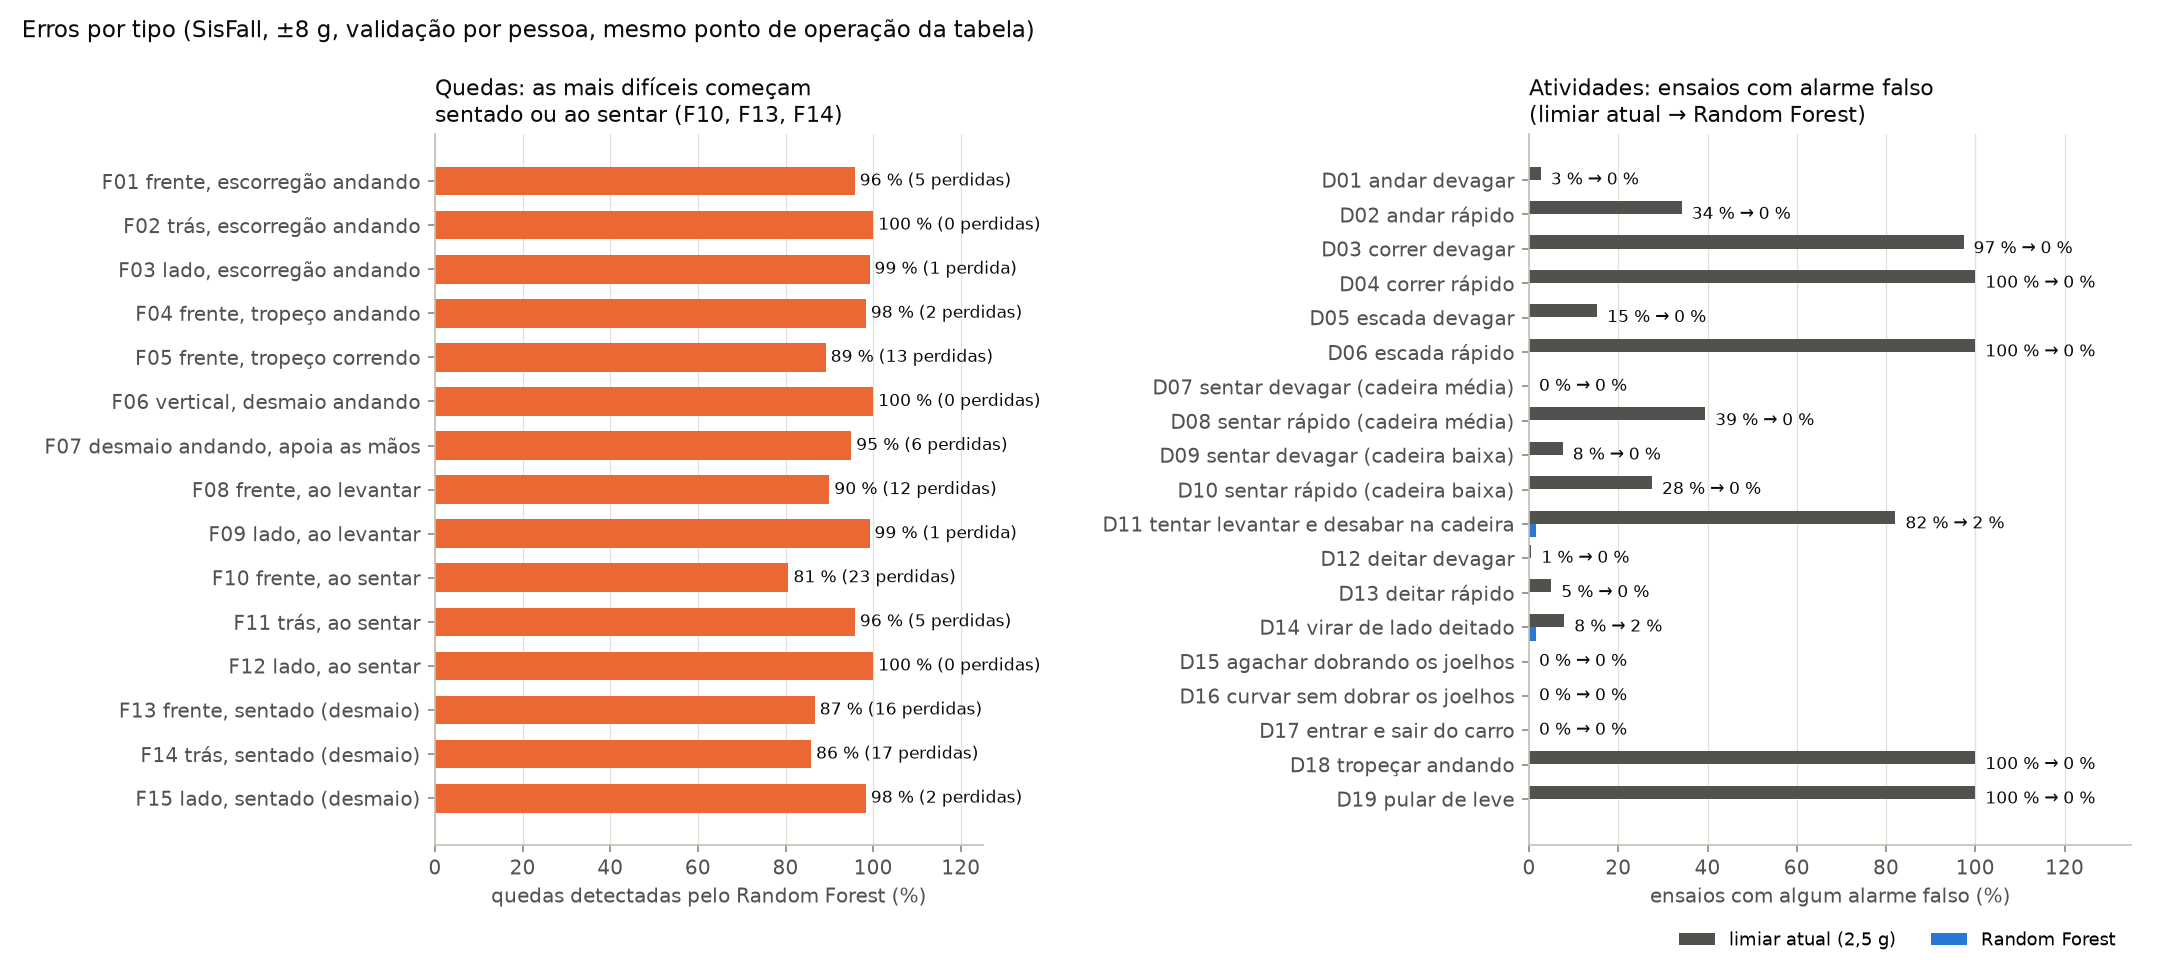
\includegraphics[width=\linewidth]{figuras/fig_erros_tipo.png}
  \caption{À esquerda, quedas detectadas pelo Random Forest por tipo. À direita, a
  fração dos ensaios de cada atividade com algum alarme falso, no limiar atual (cinza)
  e no Random Forest (azul), no cenário A.}
  \label{fig:erros}
\end{figure}

\subsection{Custo no ESP32-S3}
A Figura~\ref{fig:custo} cruza a acurácia com o tamanho estimado do modelo:
\begin{itemize}[leftmargin=1.5em]
\item \textbf{regressão logística:} cerca de 45 mil operações por janela, quase todas
  para calcular os atributos, e 412 bytes de modelo. É o melhor custo-benefício;
\item \textbf{Random Forest:} cerca de 252\,kB, que cabem na flash do ESP32-S3;
\item \textbf{CNN 1D de 6 eixos:} cerca de 243 mil multiplicações por janela e 26\,kB;
\item \textbf{kNN:} guarda o treino inteiro (cerca de 1,55\,MB) e fica de fora, embora
  seja o mais sensível com $\le$1 alarme por hora (96,1\,\%).
\end{itemize}
Como o classificador só roda quando o gatilho dispara, o custo por janela pesa pouco:
são cerca de 860 janelas por hora de atividade intensa.

\begin{figure}[H]
  \centering
  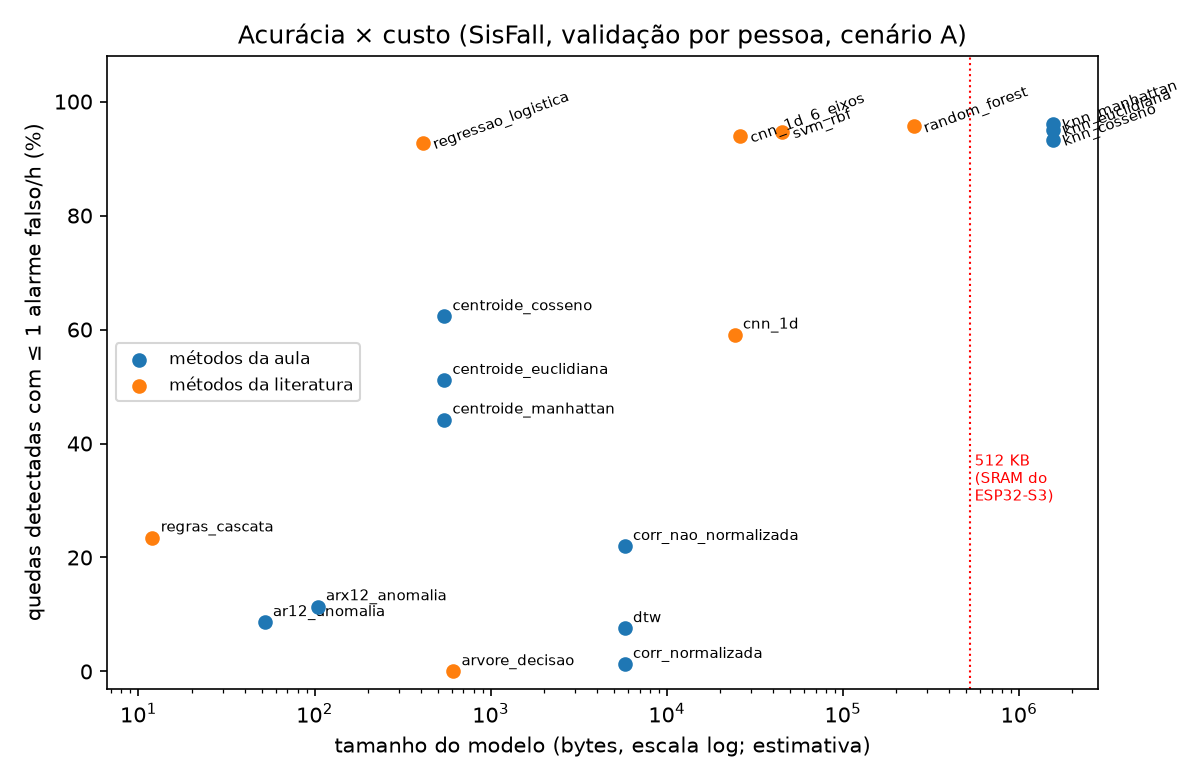
\includegraphics[width=0.9\linewidth]{figuras/fig_custo_A.png}
  \caption{Quedas detectadas com $\le$1 alarme falso por hora $\times$ tamanho
  estimado do modelo (escala log). A linha vermelha marca os 512\,KB de SRAM do
  ESP32-S3.}
  \label{fig:custo}
\end{figure}

\subsection{Nossos ensaios}
Os modelos foram treinados na SisFall saturada no cenário B, com o limiar de operação
tirado da própria SisFall, e aplicados sem ajuste aos nossos 18 ensaios. Os atributos de
correlação entre eixos ficaram de fora, porque dependem de como a placa está presa, e
nossa placa e a da SisFall têm os eixos em direções diferentes.

\begin{table}[H]
\centering
\caption{Teste externo nos nossos 18 ensaios (uma pessoa, cintura, $\pm$2\,g): modelos treinados só na SisFall saturada no cenário B, com o limiar de operação tirado da SisFall. Alarmes falsos: disparos classificados como queda nos 8 ensaios de andar e correr.}
\label{tab:proprios}
\small
\setlength{\tabcolsep}{4pt}
\begin{tabular}{@{}lccc@{}}
\toprule
Método & \makecell{Quedas\\detectadas} & \makecell{Alarmes\\falsos} & \makecell{Ensaios de atividade\\com alarme} \\
\midrule
Limiar atual (2,5\,g) & 10/10 & 8 & 8 de 8 \\
Regras em cascata & 8/10 & 5 & 4 de 8 \\
Correlação normalizada & 10/10 & 12 & 6 de 8 \\
DTW & 10/10 & 8 & 6 de 8 \\
AR(12) como anomalia & 10/10 & 18 & 8 de 8 \\
Centroide (cosseno) & 8/10 & 4 & 3 de 8 \\
kNN (Manhattan) & 8/10 & 1 & 1 de 8 \\
Regressão logística & 7/10 & 0 & 0 de 8 \\
SVM (RBF) & 8/10 & 0 & 0 de 8 \\
Random Forest & 7/10 & 0 & 0 de 8 \\
CNN 1D (módulos) & 9/10 & 12 & 7 de 8 \\
\bottomrule
\end{tabular}
\end{table}


O limiar atual detecta as 10 quedas, mas dá alarme em todos os 8 ensaios de andar e
correr. Random Forest, regressão logística e SVM não dão nenhum alarme falso e detectam
todas as quedas de frente e de costas, mas perdem as quedas de joelhos
(Figuras~\ref{fig:proprios_matriz} e \ref{fig:proprios_ensaios}). Essas quedas são mais
lentas, não têm equivalente direto na SisFall, e os ensaios acabam cerca de 1\,s depois
do impacto, antes que a postura final apareça na janela.

\begin{figure}[H]
  \centering
  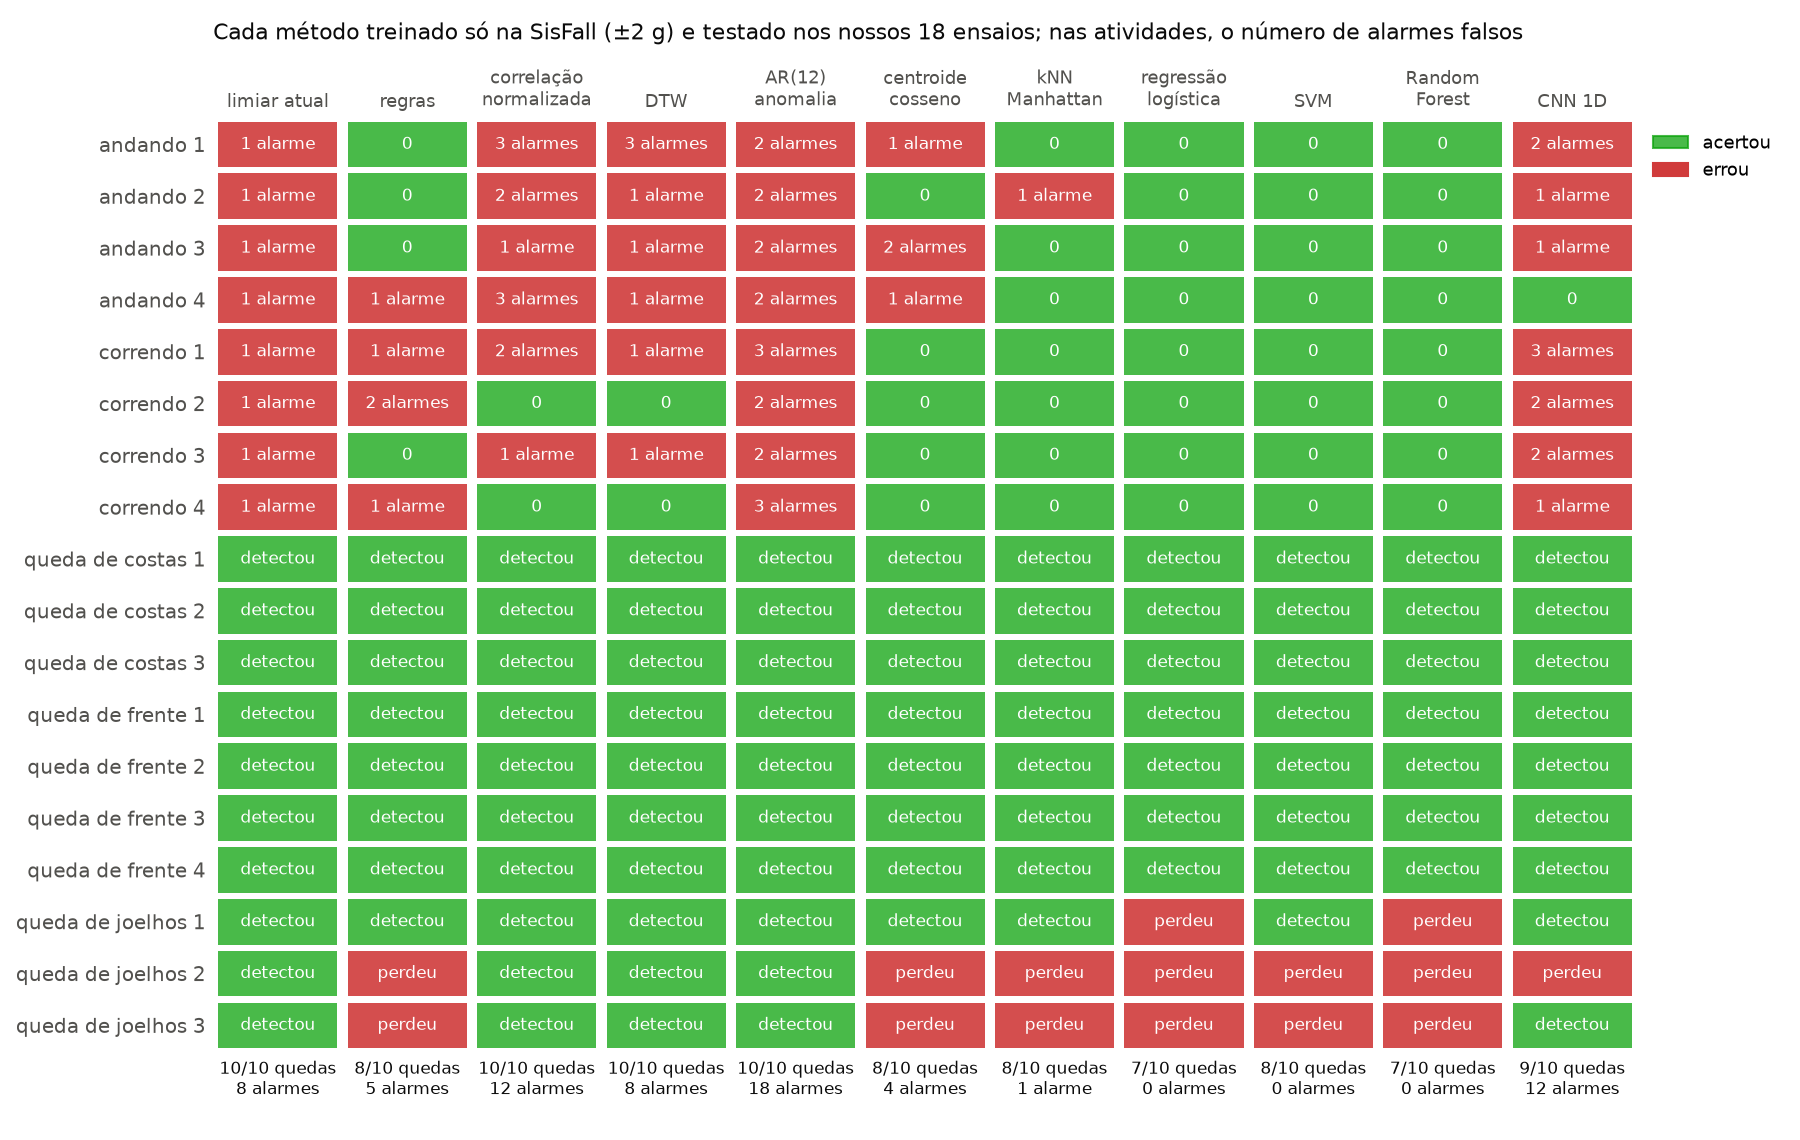
\includegraphics[width=\linewidth]{figuras/fig_proprios_matriz.png}
  \caption{Resultado de cada método em cada um dos nossos ensaios. Nas atividades, o
  número de alarmes falsos; nas quedas, se foi detectada. Embaixo, os totais.}
  \label{fig:proprios_matriz}
\end{figure}

\begin{figure}[H]
  \centering
  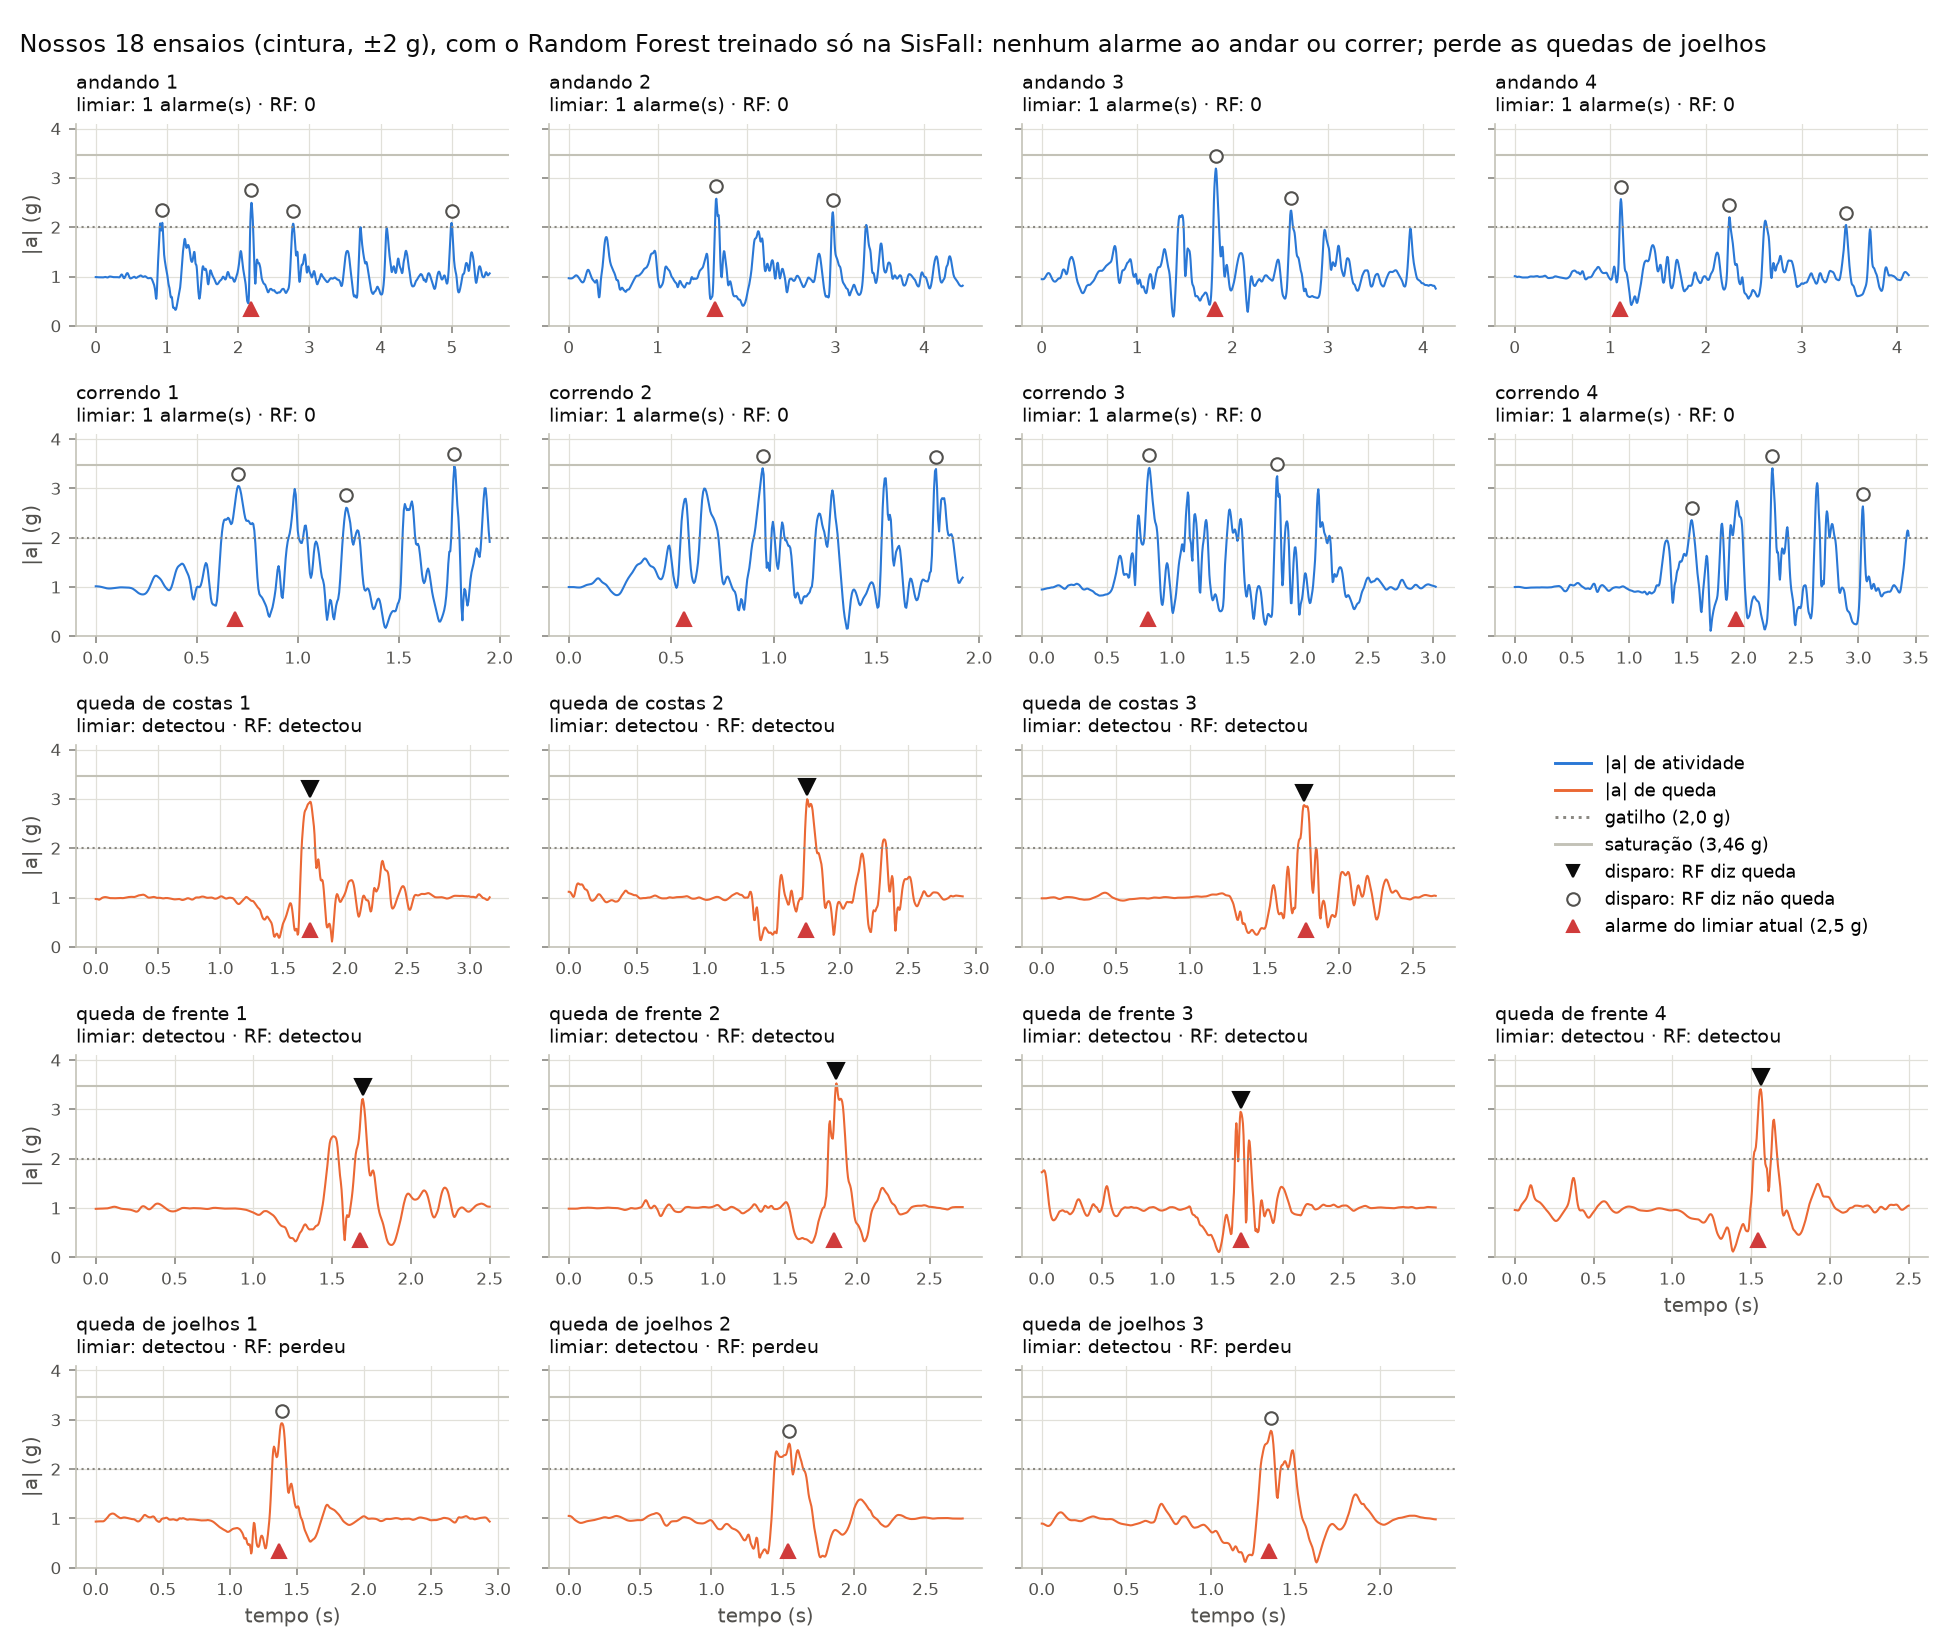
\includegraphics[width=\linewidth]{figuras/fig_proprios_ensaios.png}
  \caption{Os 18 ensaios ($\amag$ filtrado, saturado em 3,46\,g), com cada disparo do
  gatilho e a decisão do Random Forest (triângulo preto: queda; círculo: não queda) e
  os alarmes do limiar atual (triângulo vermelho).}
  \label{fig:proprios_ensaios}
\end{figure}

%======================================================================
\section{Discussão}\label{sec:discussao}
%======================================================================
\begin{itemize}[leftmargin=1.5em]
\item \textbf{O limiar serve como gatilho, não como decisão.} Ele deixa passar 99\,\%
  das quedas e reduz o trabalho do classificador a uma janela a cada cerca de 4\,s de
  atividade intensa; decidindo sozinho, dá cerca de 70 alarmes falsos por hora.
\item \textbf{O que separa queda de atividade é o contexto do impacto:} a queda livre
  antes e a postura e a quietude depois. Por isso os atributos no tempo vencem, e a CNN
  só com os módulos (59,1\,\% com $\le$1 alarme por hora) perde para a de 6 eixos
  (93,9\,\%): sem os eixos, ela não vê a inclinação mudar.
\item \textbf{Os métodos dos slides:} comparar formas de onda (correlação, DTW) e o AR
  como detector de anomalia ficam bem atrás, porque correr e tropeçar também têm um pico
  curto e imprevisível. As distâncias entre vetores de atributos vão bem: o kNN com
  distância de Manhattan é o mais sensível com poucos alarmes, mas não cabe no ESP32.
\item \textbf{O modelo autorregressivo} descreve e prevê bem o sinal normal, mas o erro
  de predição não é específico da queda. O AR é mais útil para modelar o sinal do que
  para classificar a queda; como atributo, sozinho, também é fraco.
\item \textbf{A faixa do sensor importa:} em $\pm$2\,g, os métodos que dependem do pico
  e da energia perdem muito. O vestível deve continuar em $\pm$8\,g.
\item \textbf{Recomendação para o ESP32:} começar pela regressão logística (412 bytes,
  92,8\,\% das quedas com $\le$1 alarme por hora) e depois levar o Random Forest
  (95,7\,\%), gerado em C a partir do modelo treinado em Python.
\end{itemize}

%======================================================================
\section{Conclusões}\label{sec:conclusoes}
%======================================================================
\begin{itemize}[leftmargin=1.5em]
\item Desenvolvemos e comparamos 22 métodos de detecção de queda, todos depois do mesmo
  pipeline (filtro, gatilho de picos em 2,0\,g e janela de 1,8\,s), com validação
  cruzada por pessoa na SisFall e teste externo nos nossos ensaios.
\item Com cerca de 94\,\% das quedas detectadas, o Random Forest dá 0,4 alarme falso por
  hora de atividade e a regressão logística, 1,4, contra 69,9 do limiar atual.
\item O modelo autorregressivo, pedido pelo enunciado, foi implementado como detector
  de anomalia (AR e ARX, ordem pelo BIC) e como atributo. Ele descreve bem a atividade
  normal, mas não separa a queda de outros movimentos bruscos.
\item Nos nossos ensaios, os melhores modelos não deram nenhum alarme ao andar ou correr
  e detectaram as quedas de frente e de costas; perderam as quedas de joelhos.
\end{itemize}

\subsection{Limitações}
\begin{itemize}[leftmargin=1.5em]
\item O vestível final é uma pulseira, mas os dados (SisFall e os nossos) são da
  cintura. No pulso, o braço se move muito mais, e os resultados não se transferem sem
  dados de pulso.
\item Nossos ensaios: uma pessoa, 18 ensaios curtos, em $\pm$2\,g.
\item Na SisFall, as quedas são simuladas por jovens; os idosos só fazem atividades.
\item O limiar de operação foi tirado dos escores da própria validação. Ele serve para
  comparar os métodos; o limiar do vestível precisa sair de uma validação separada.
\end{itemize}

\subsection{Próximos passos}
\begin{enumerate}[leftmargin=1.8em]
\item Nova coleta com o firmware atual, no pulso, em $\pm$8\,g e $\pm$500\,°/s, com
  várias pessoas e ensaios de pelo menos 10\,s.
\item Pipeline no ESP32: biquad, gatilho de picos, janela do buffer circular,
  atributos e classificador, rodando só quando o gatilho dispara; vetores de teste do
  Python para conferir que o C dá os mesmos atributos e a mesma decisão.
\item Limiar de operação calibrado numa validação separada.
\end{enumerate}

%======================================================================
\phantomsection
\addcontentsline{toc}{section}{Referências}
\begin{thebibliography}{9}
\bibitem{sisfall} SUCERQUIA, A.; LÓPEZ, J. D.; VARGAS-BONILLA, J. F. SisFall: a fall
  and movement dataset. \emph{Sensors}, v.~17, n.~1, p.~198, 2017.
\bibitem{slides} Slides da disciplina: ``ESP32 - Modelos Autoregressivos'', ``ESP32 -
  Segmentação e atributos'' e ``ESP32 - TDF''. Escola Politécnica da USP, 2026.
\bibitem{box} BOX, G. E. P.; JENKINS, G. M.; REINSEL, G. C.; LJUNG, G. M. \emph{Time
  series analysis: forecasting and control}. 5.~ed. Hoboken: Wiley, 2015.
\bibitem{akaike} AKAIKE, H. A new look at the statistical model identification.
  \emph{IEEE Transactions on Automatic Control}, v.~19, n.~6, p.~716--723, 1974.
\bibitem{schwarz} SCHWARZ, G. Estimating the dimension of a model. \emph{The Annals of
  Statistics}, v.~6, n.~2, p.~461--464, 1978.
\bibitem{sakoe} SAKOE, H.; CHIBA, S. Dynamic programming algorithm optimization for
  spoken word recognition. \emph{IEEE Transactions on Acoustics, Speech, and Signal
  Processing}, v.~26, n.~1, p.~43--49, 1978.
\bibitem{breiman} BREIMAN, L. Random forests. \emph{Machine Learning}, v.~45, n.~1,
  p.~5--32, 2001.
\bibitem{sklearn} PEDREGOSA, F. et al. Scikit-learn: machine learning in Python.
  \emph{Journal of Machine Learning Research}, v.~12, p.~2825--2830, 2011.
\bibitem{pytorch} PASZKE, A. et al. PyTorch: an imperative style, high-performance deep
  learning library. In: \emph{Advances in Neural Information Processing Systems 32}, 2019.
\end{thebibliography}

%======================================================================
\appendix
\section{Reprodução dos resultados}\label{ap:reproducao}
O código está na pasta \code{modelo/} do repositório do projeto:
\begin{itemize}[leftmargin=1.5em]
\item \code{queda/dados.py}: leitura da SisFall e dos nossos ensaios, saturação;
\item \code{queda/pipeline.py}: filtro, gatilho, janelas e cenários;
\item \code{queda/atributos.py}: atributos no tempo, FFT e AR por mínimos quadrados;
\item \code{queda/modelos.py} e \code{queda/cnn.py}: os modelos da
  Seção~\ref{sec:modelos};
\item \code{queda/avaliacao.py}: dobras por pessoa, métricas e linha de base;
\item \code{tests/}: os testes da Tabela~\ref{tab:testes};
\item \code{experimentos/}: os scripts, numerados na ordem de execução.
\end{itemize}
Com o gerenciador \code{uv} (Python~3.12, scikit-learn, statsmodels, PyTorch para CPU),
em \code{modelo/}:
\begin{verbatim}
uv sync
uv run pytest
uv run python experimentos/02_gatilho.py
uv run python experimentos/03_comparar.py --cenario A
uv run python experimentos/03_comparar.py --cenario B
uv run python experimentos/04_dados_proprios.py
uv run python experimentos/01_explorar.py
uv run python experimentos/05_figuras.py
uv run python experimentos/06_resumo.py
uv run python experimentos/07_figuras_explicativas.py
uv run python experimentos/08_relatorio_latex.py
\end{verbatim}
O último script copia as figuras para \code{figuras/} e gera as tabelas de
\code{tabelas/} a partir dos resultados, de modo que nenhum número das tabelas é
digitado à mão. O relatório é compilado com \code{pdflatex main.tex} (duas vezes, por
causa do sumário).

\end{document}
